\appendix{Представление графического материала}

Графический материал, выполненный на отдельных листах,
изображен на рисунках А.1--А.\arabic{числоПлакатов}.
\setcounter{числоПлакатов}{0}

\renewcommand{\thefigure}{А.\arabic{figure}} % шаблон номера для плакатов

\begin{landscape}

\begin{плакат}
    
\includegraphics[width=0.82\linewidth]{posters/p1.eps}
    \заголовок{Сведения о ВКРБ}
    \label{p1:image}      
\end{плакат}

\begin{плакат}
    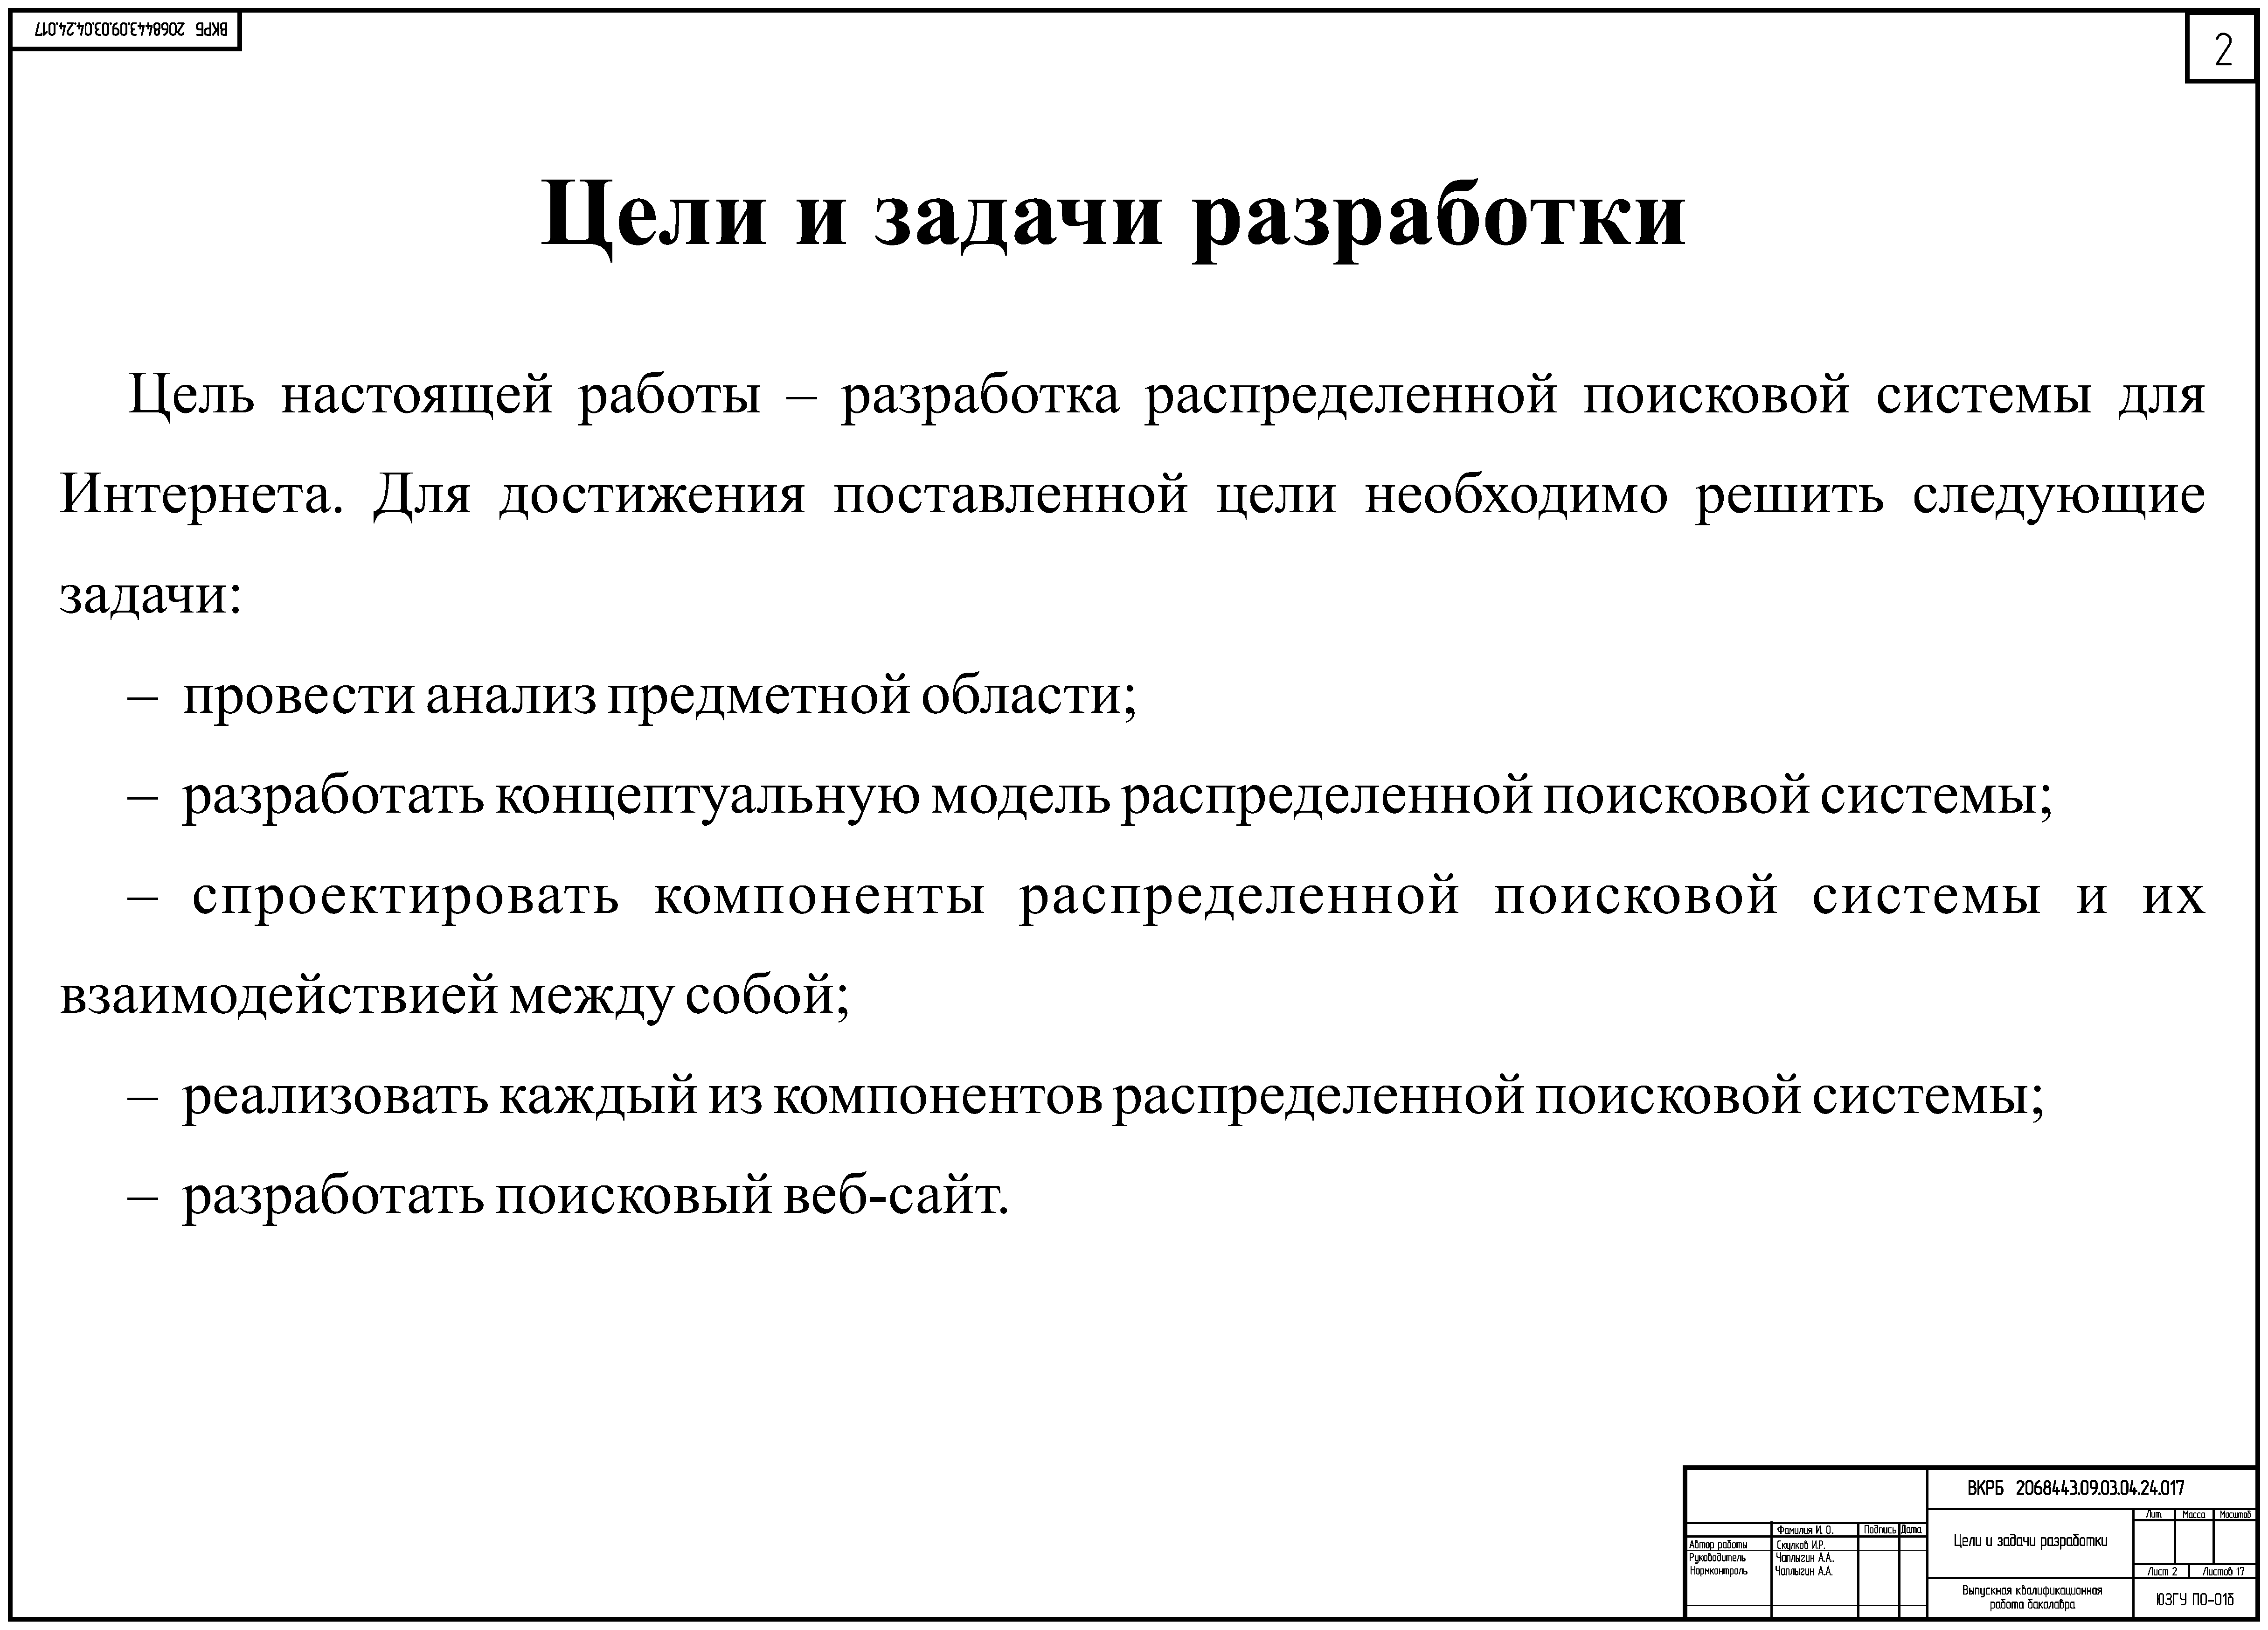
\includegraphics[width=0.82\linewidth]{posters/p2.eps}
    \заголовок{Цели и задачи разработки}
    \label{p2:image}      
\end{плакат}

\begin{плакат}
    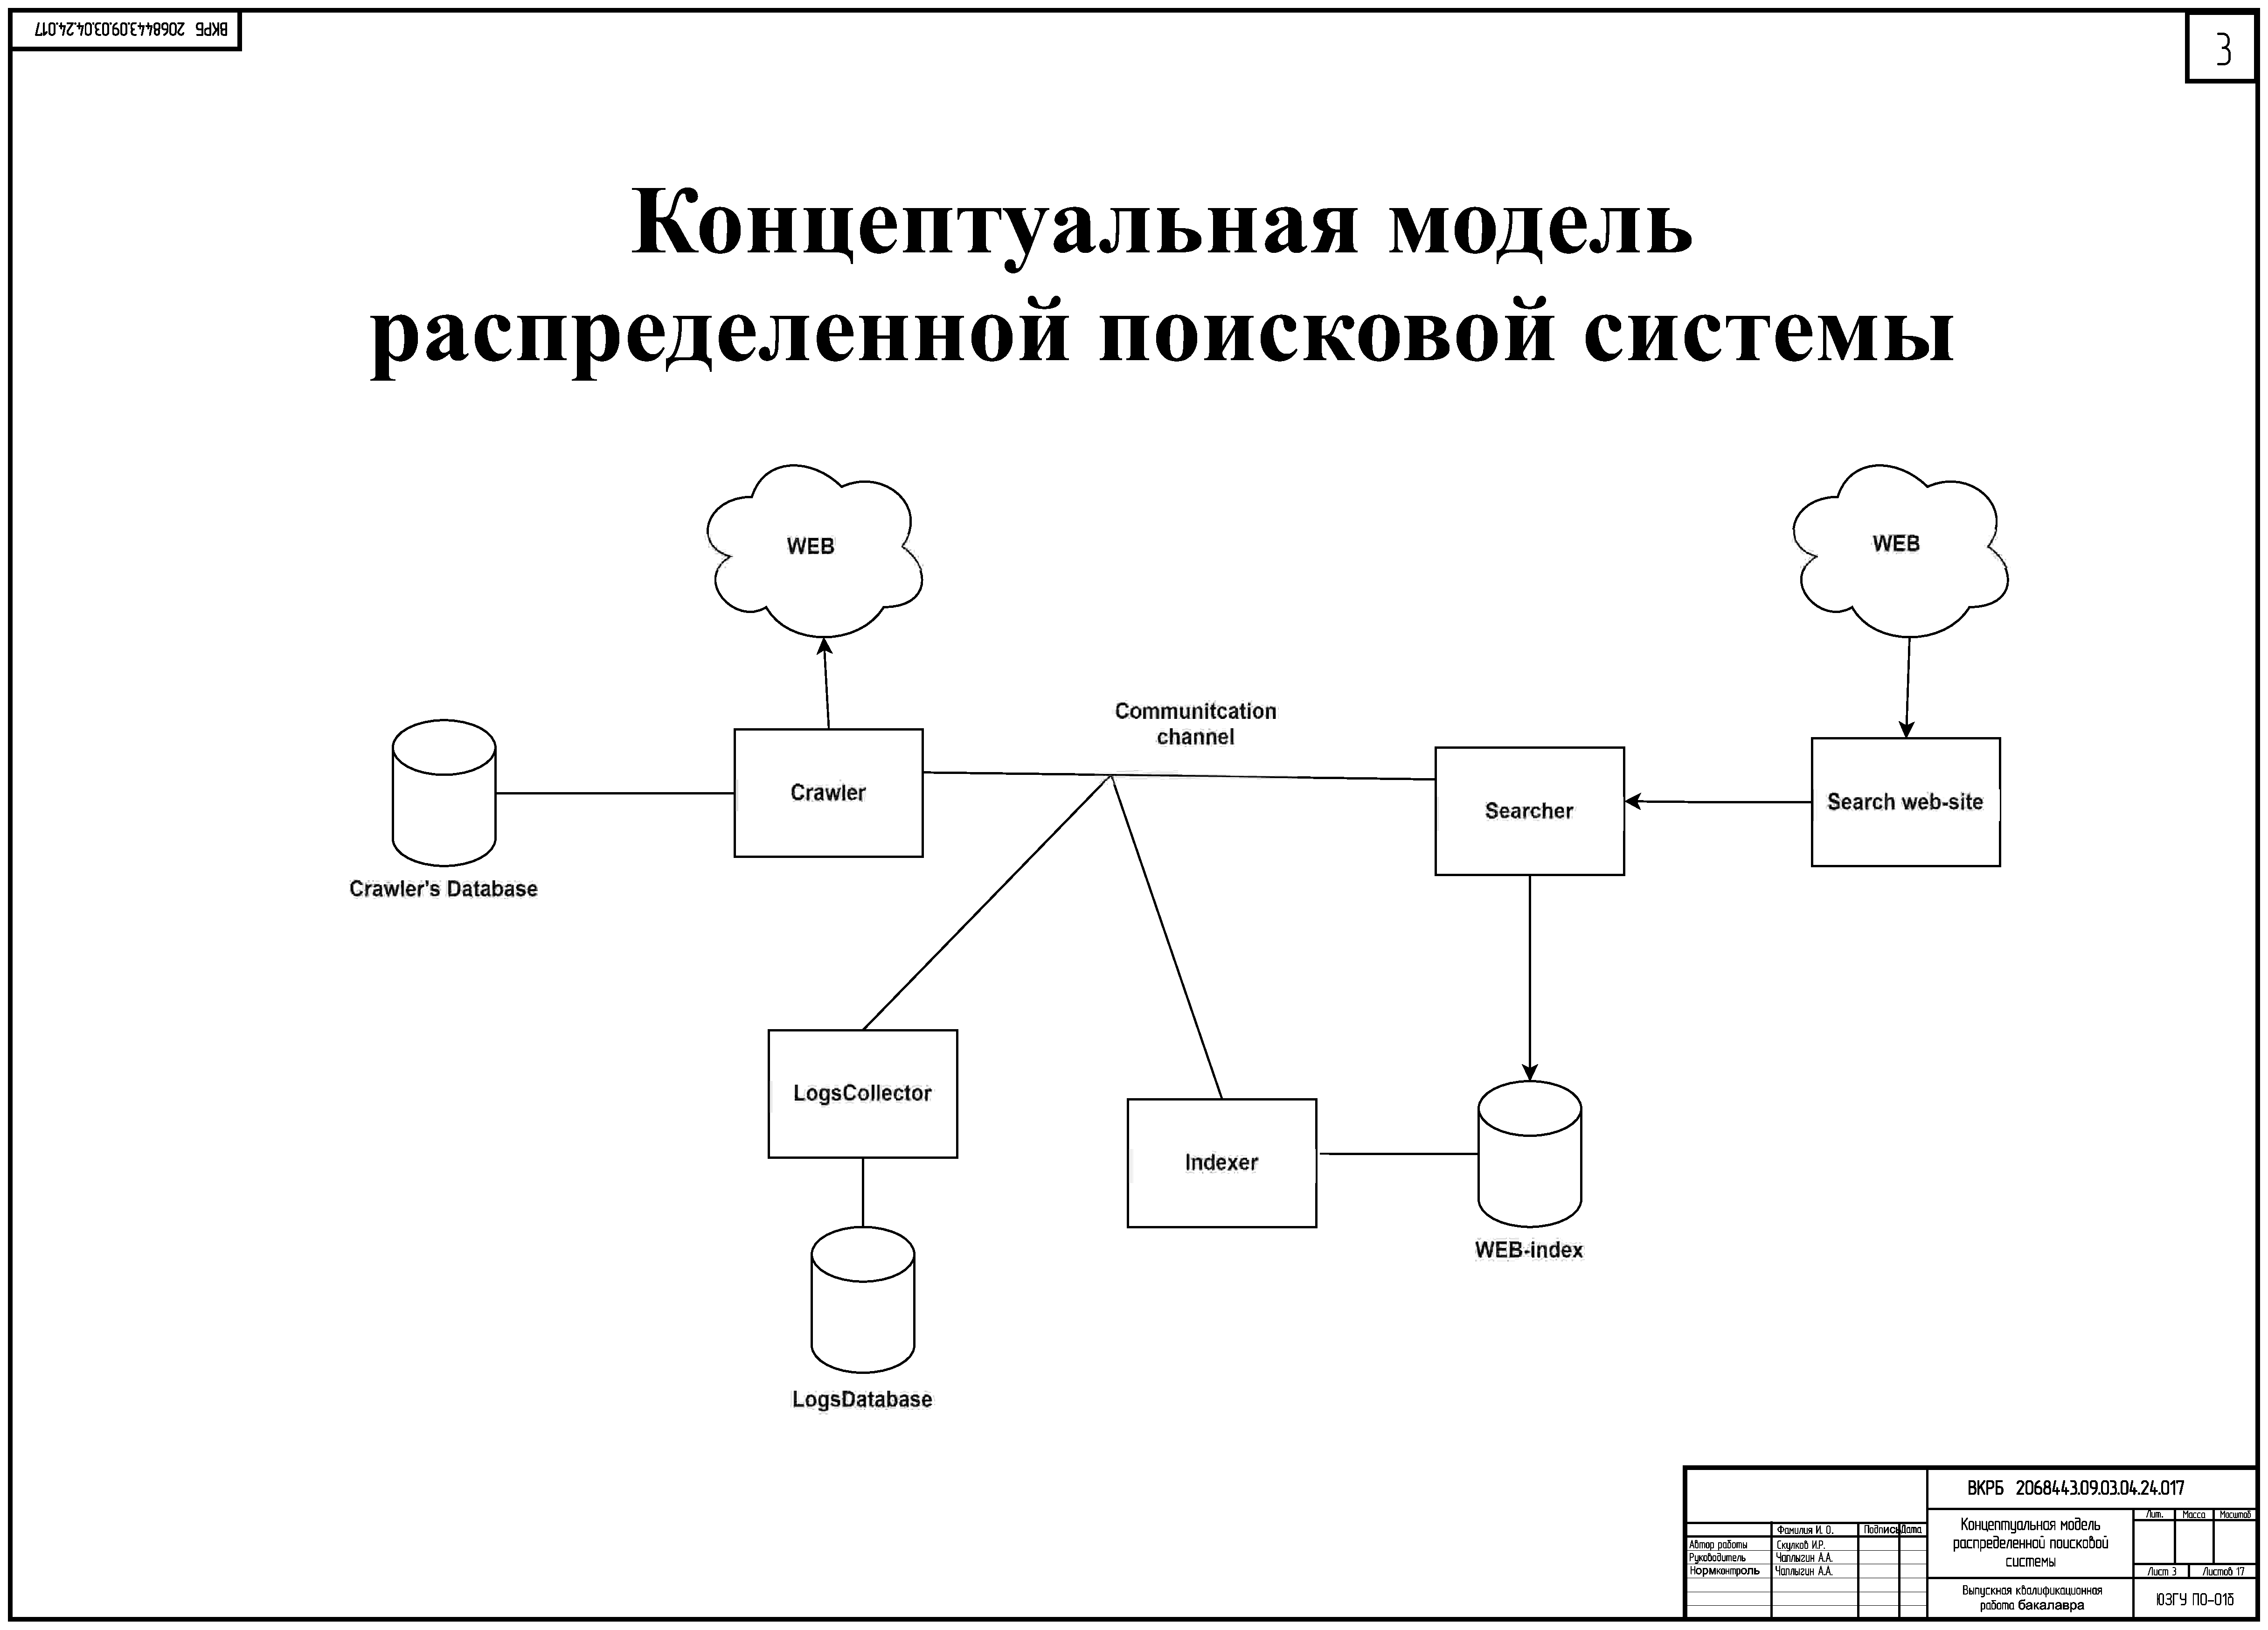
\includegraphics[width=0.82\linewidth]{posters/p3.eps}
    \заголовок{Концептуальная модель распределенной поисковой системы}
    \label{p3:image}      
\end{плакат}

\begin{плакат}
    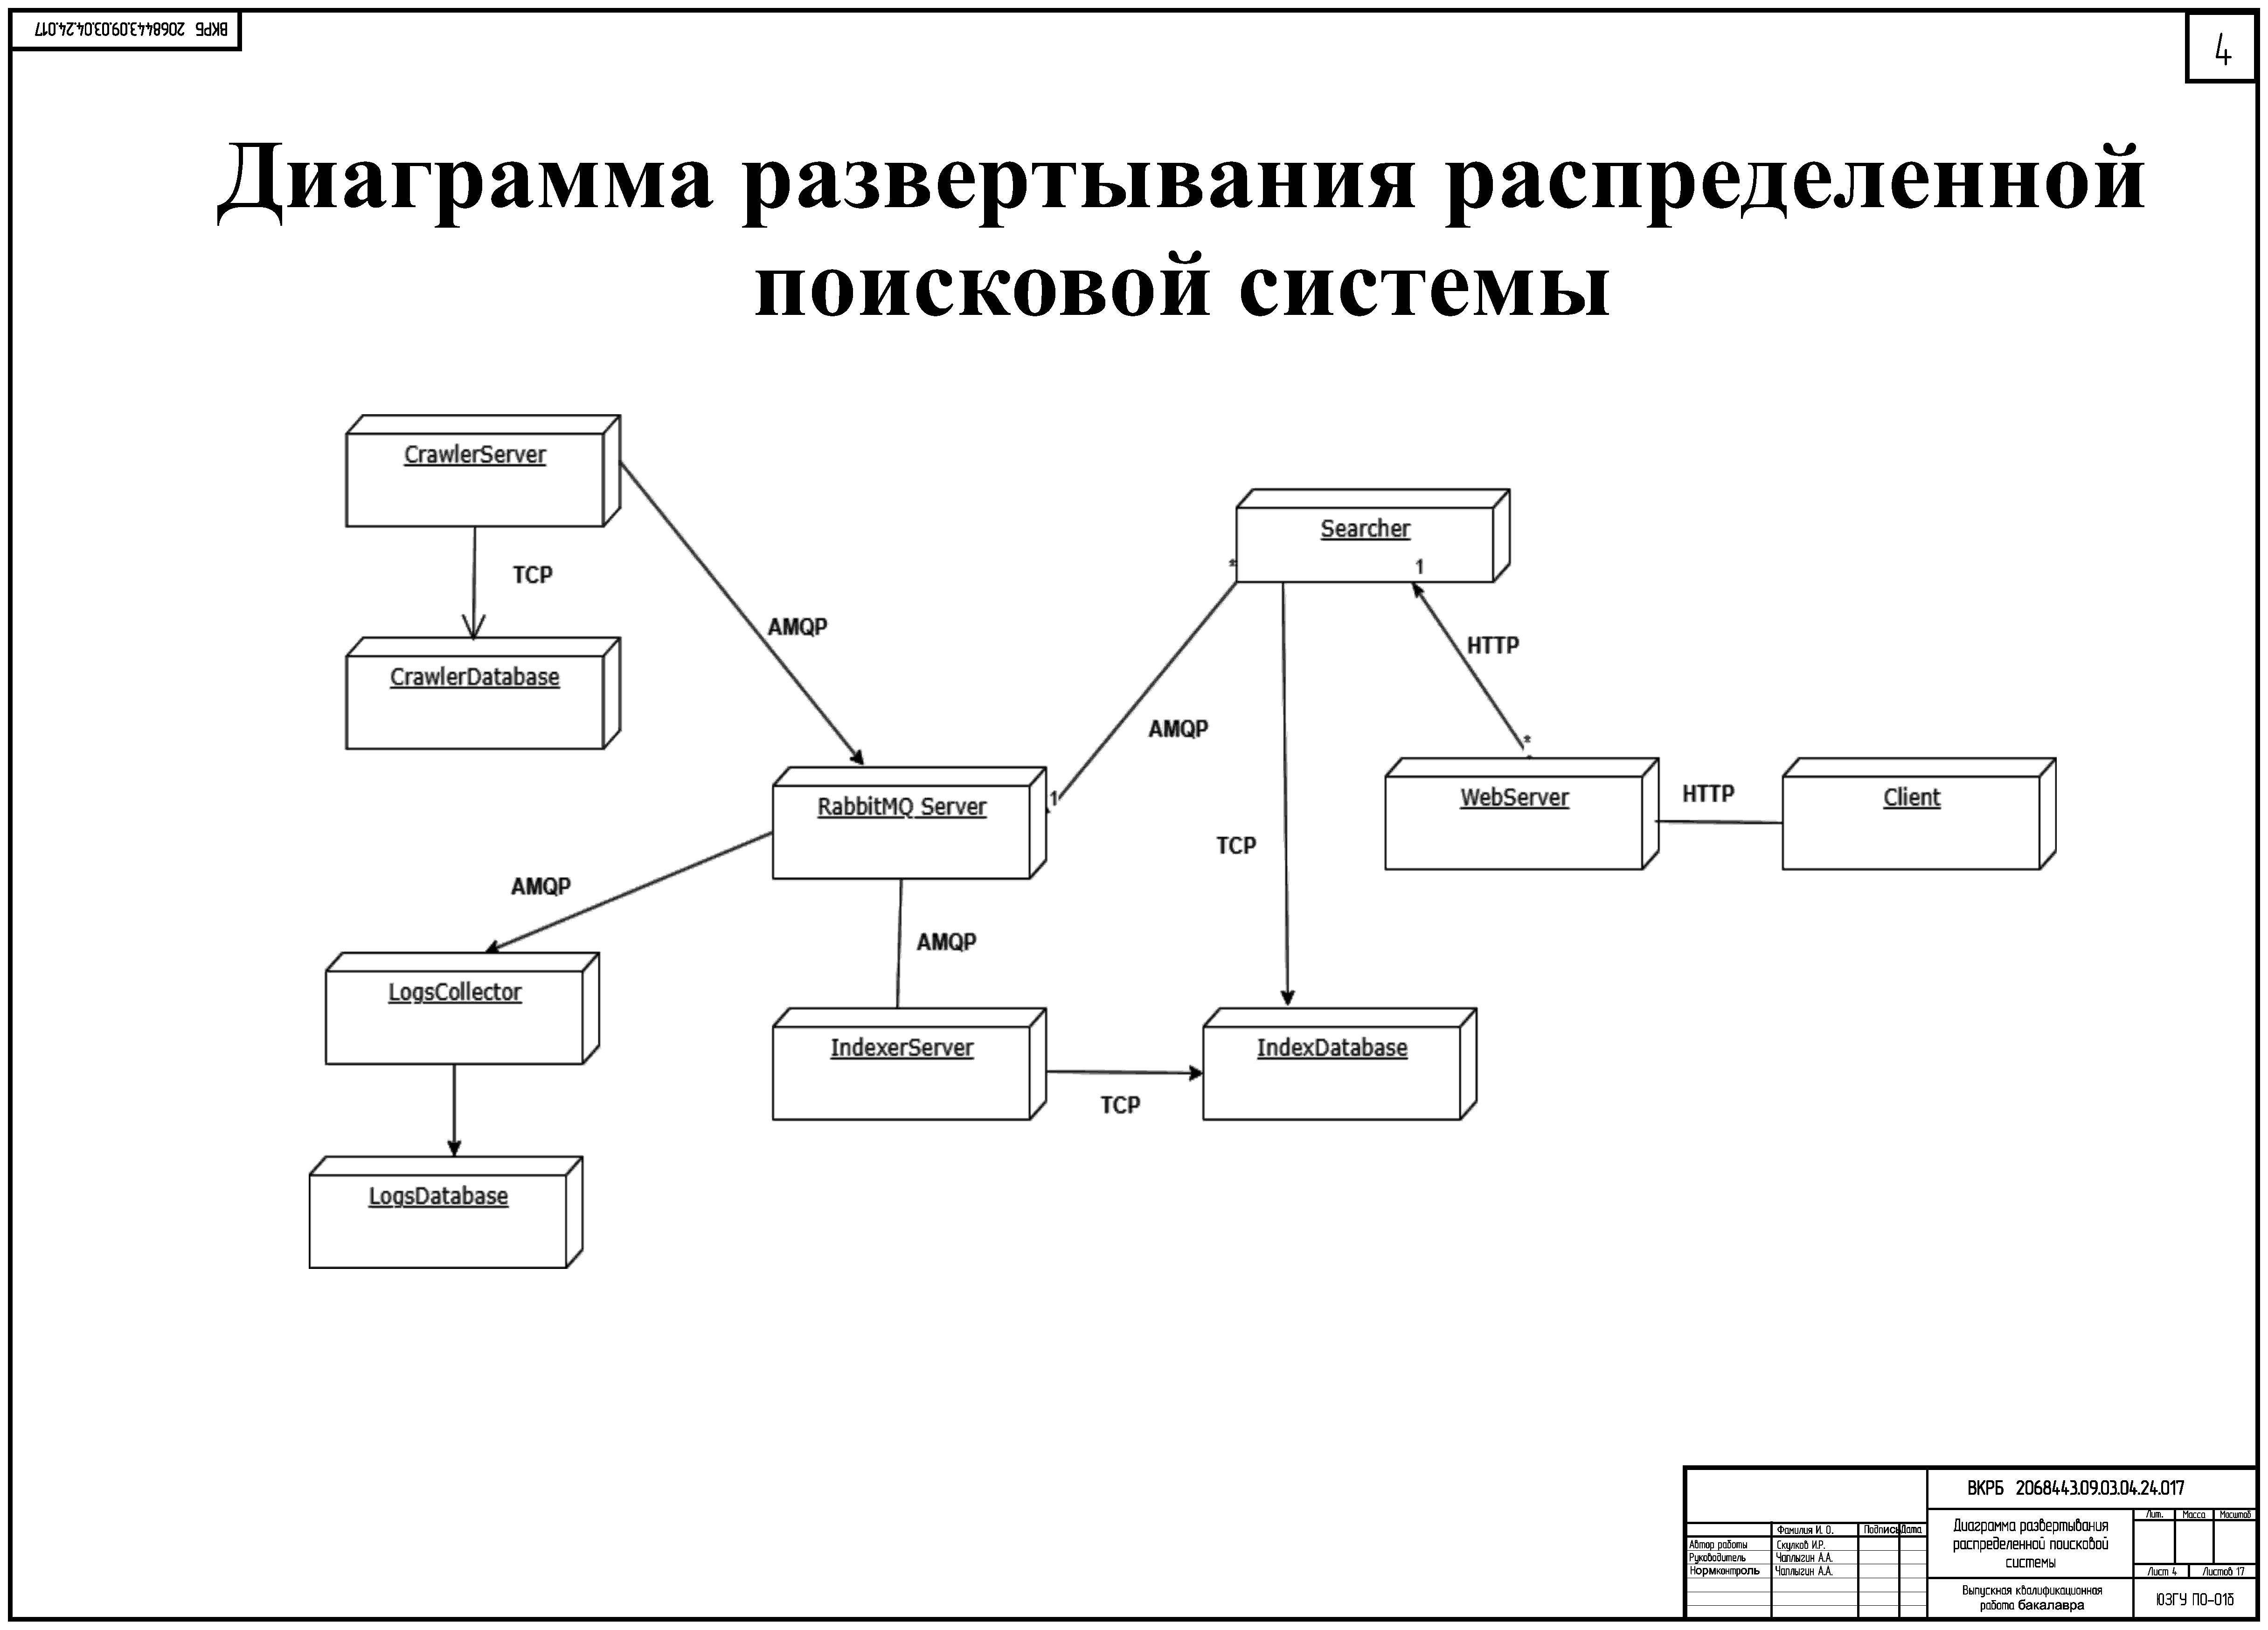
\includegraphics[width=0.82\linewidth]{posters/p4.eps}
    \заголовок{Диаграмма развертывания распределенной поисковой системы}
    \label{p4:image}      
\end{плакат}

\begin{плакат}
    
\includegraphics[width=0.82\linewidth]{posters/p5.eps}
    \заголовок{Диаграмма вариантов использования}
    \label{p5:image}      
\end{плакат}

\begin{плакат}
    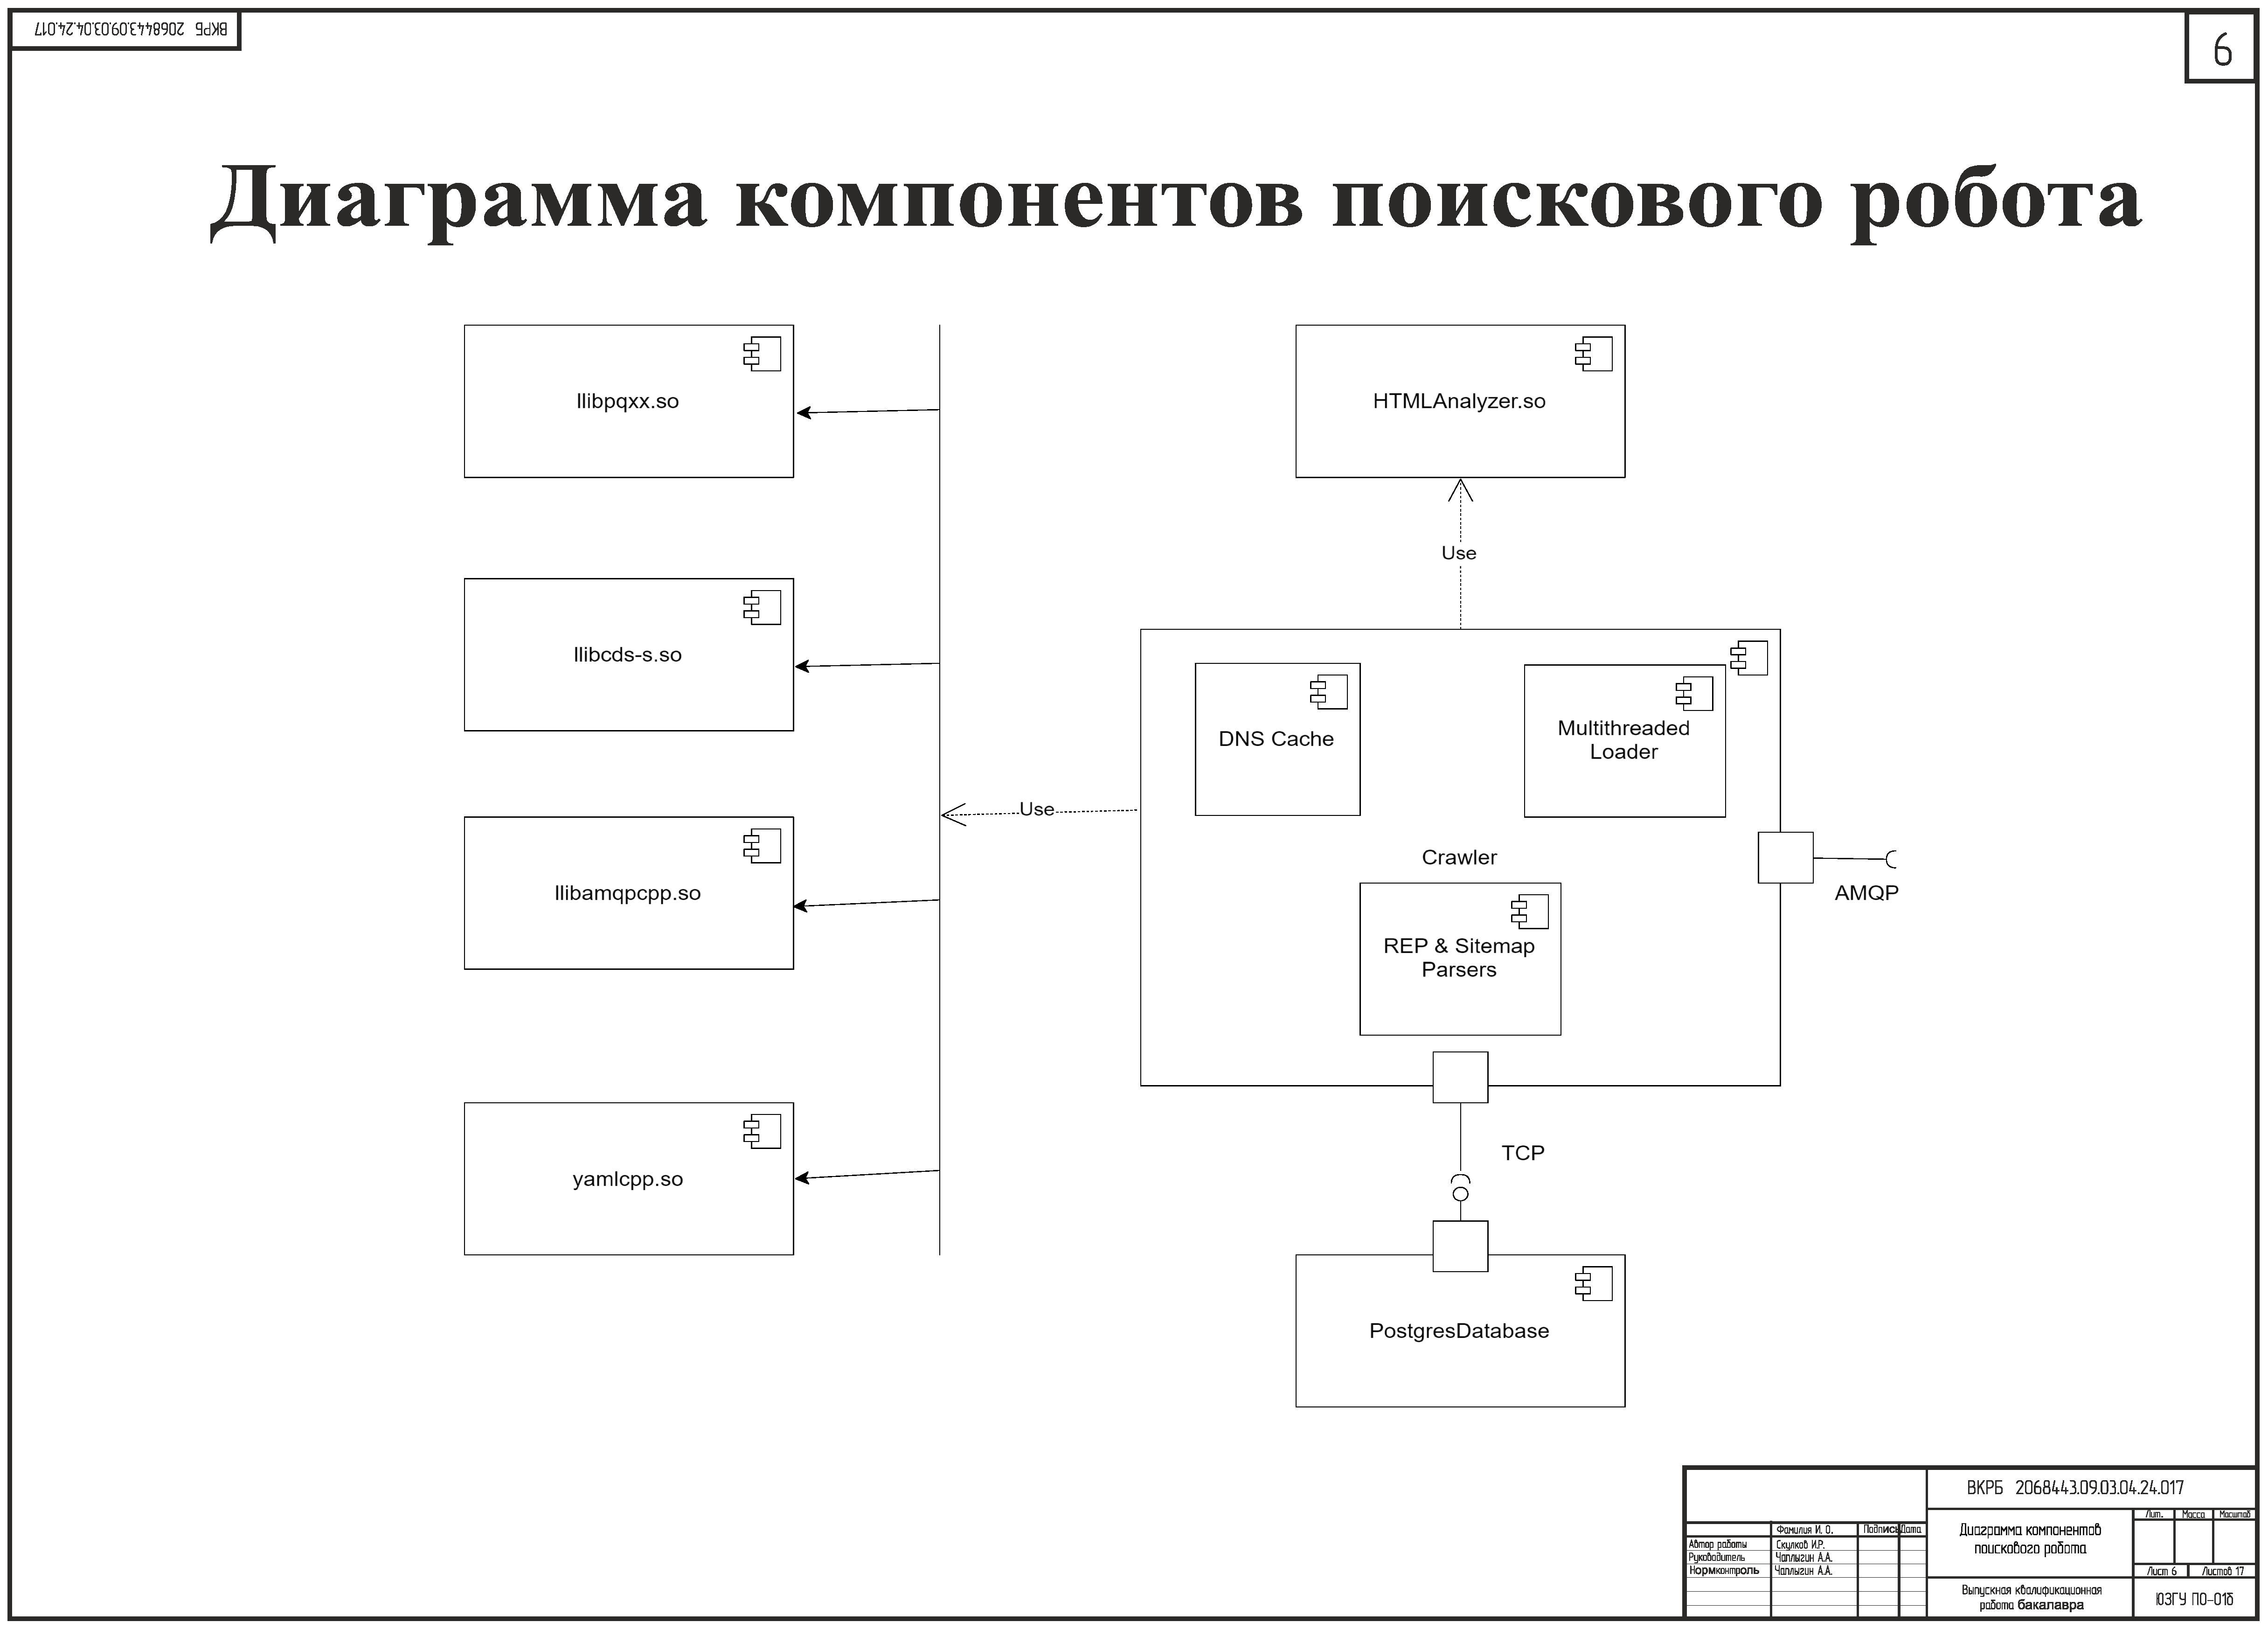
\includegraphics[width=0.82\linewidth]{posters/pr1.eps}
    \заголовок{Диаграмма компонентов поискового робота}
    \label{pr1:image}      
\end{плакат}

\begin{плакат}
    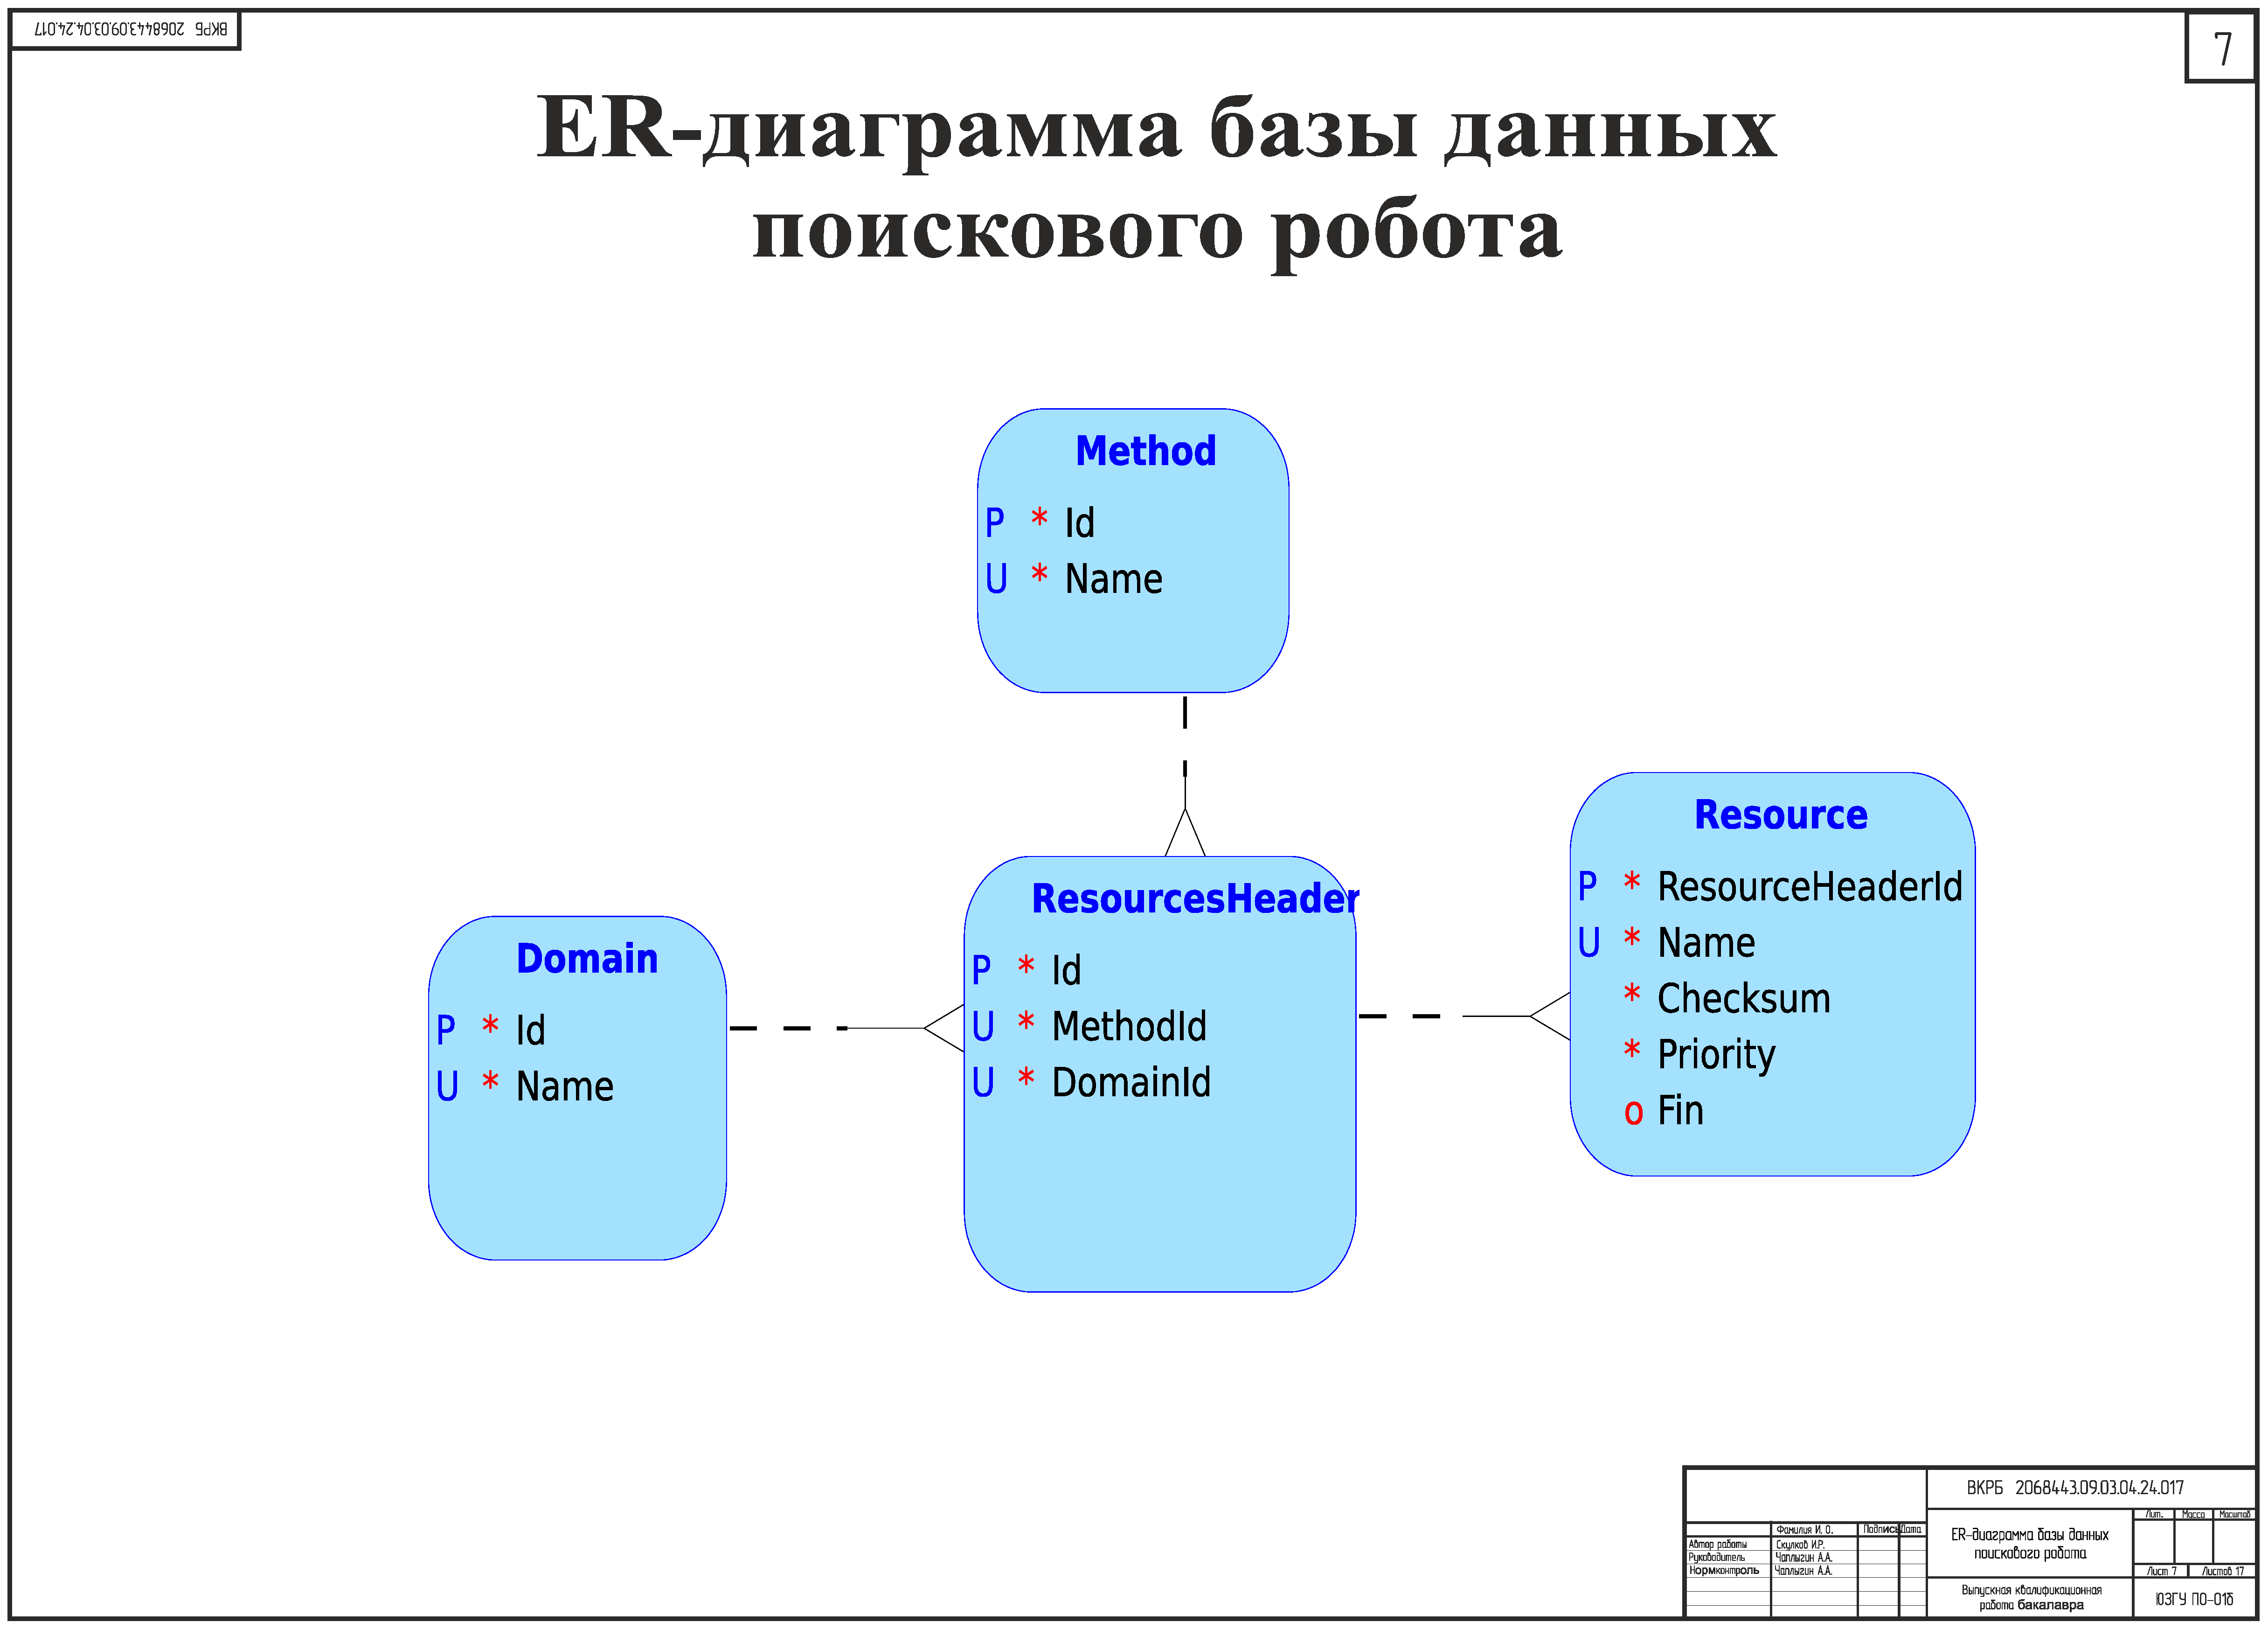
\includegraphics[width=0.82\linewidth]{posters/pr2.eps}
    \заголовок{ER-диаграмма базы данных поискового робота}
    \label{pr2:image}      
\end{плакат}

\begin{плакат}
    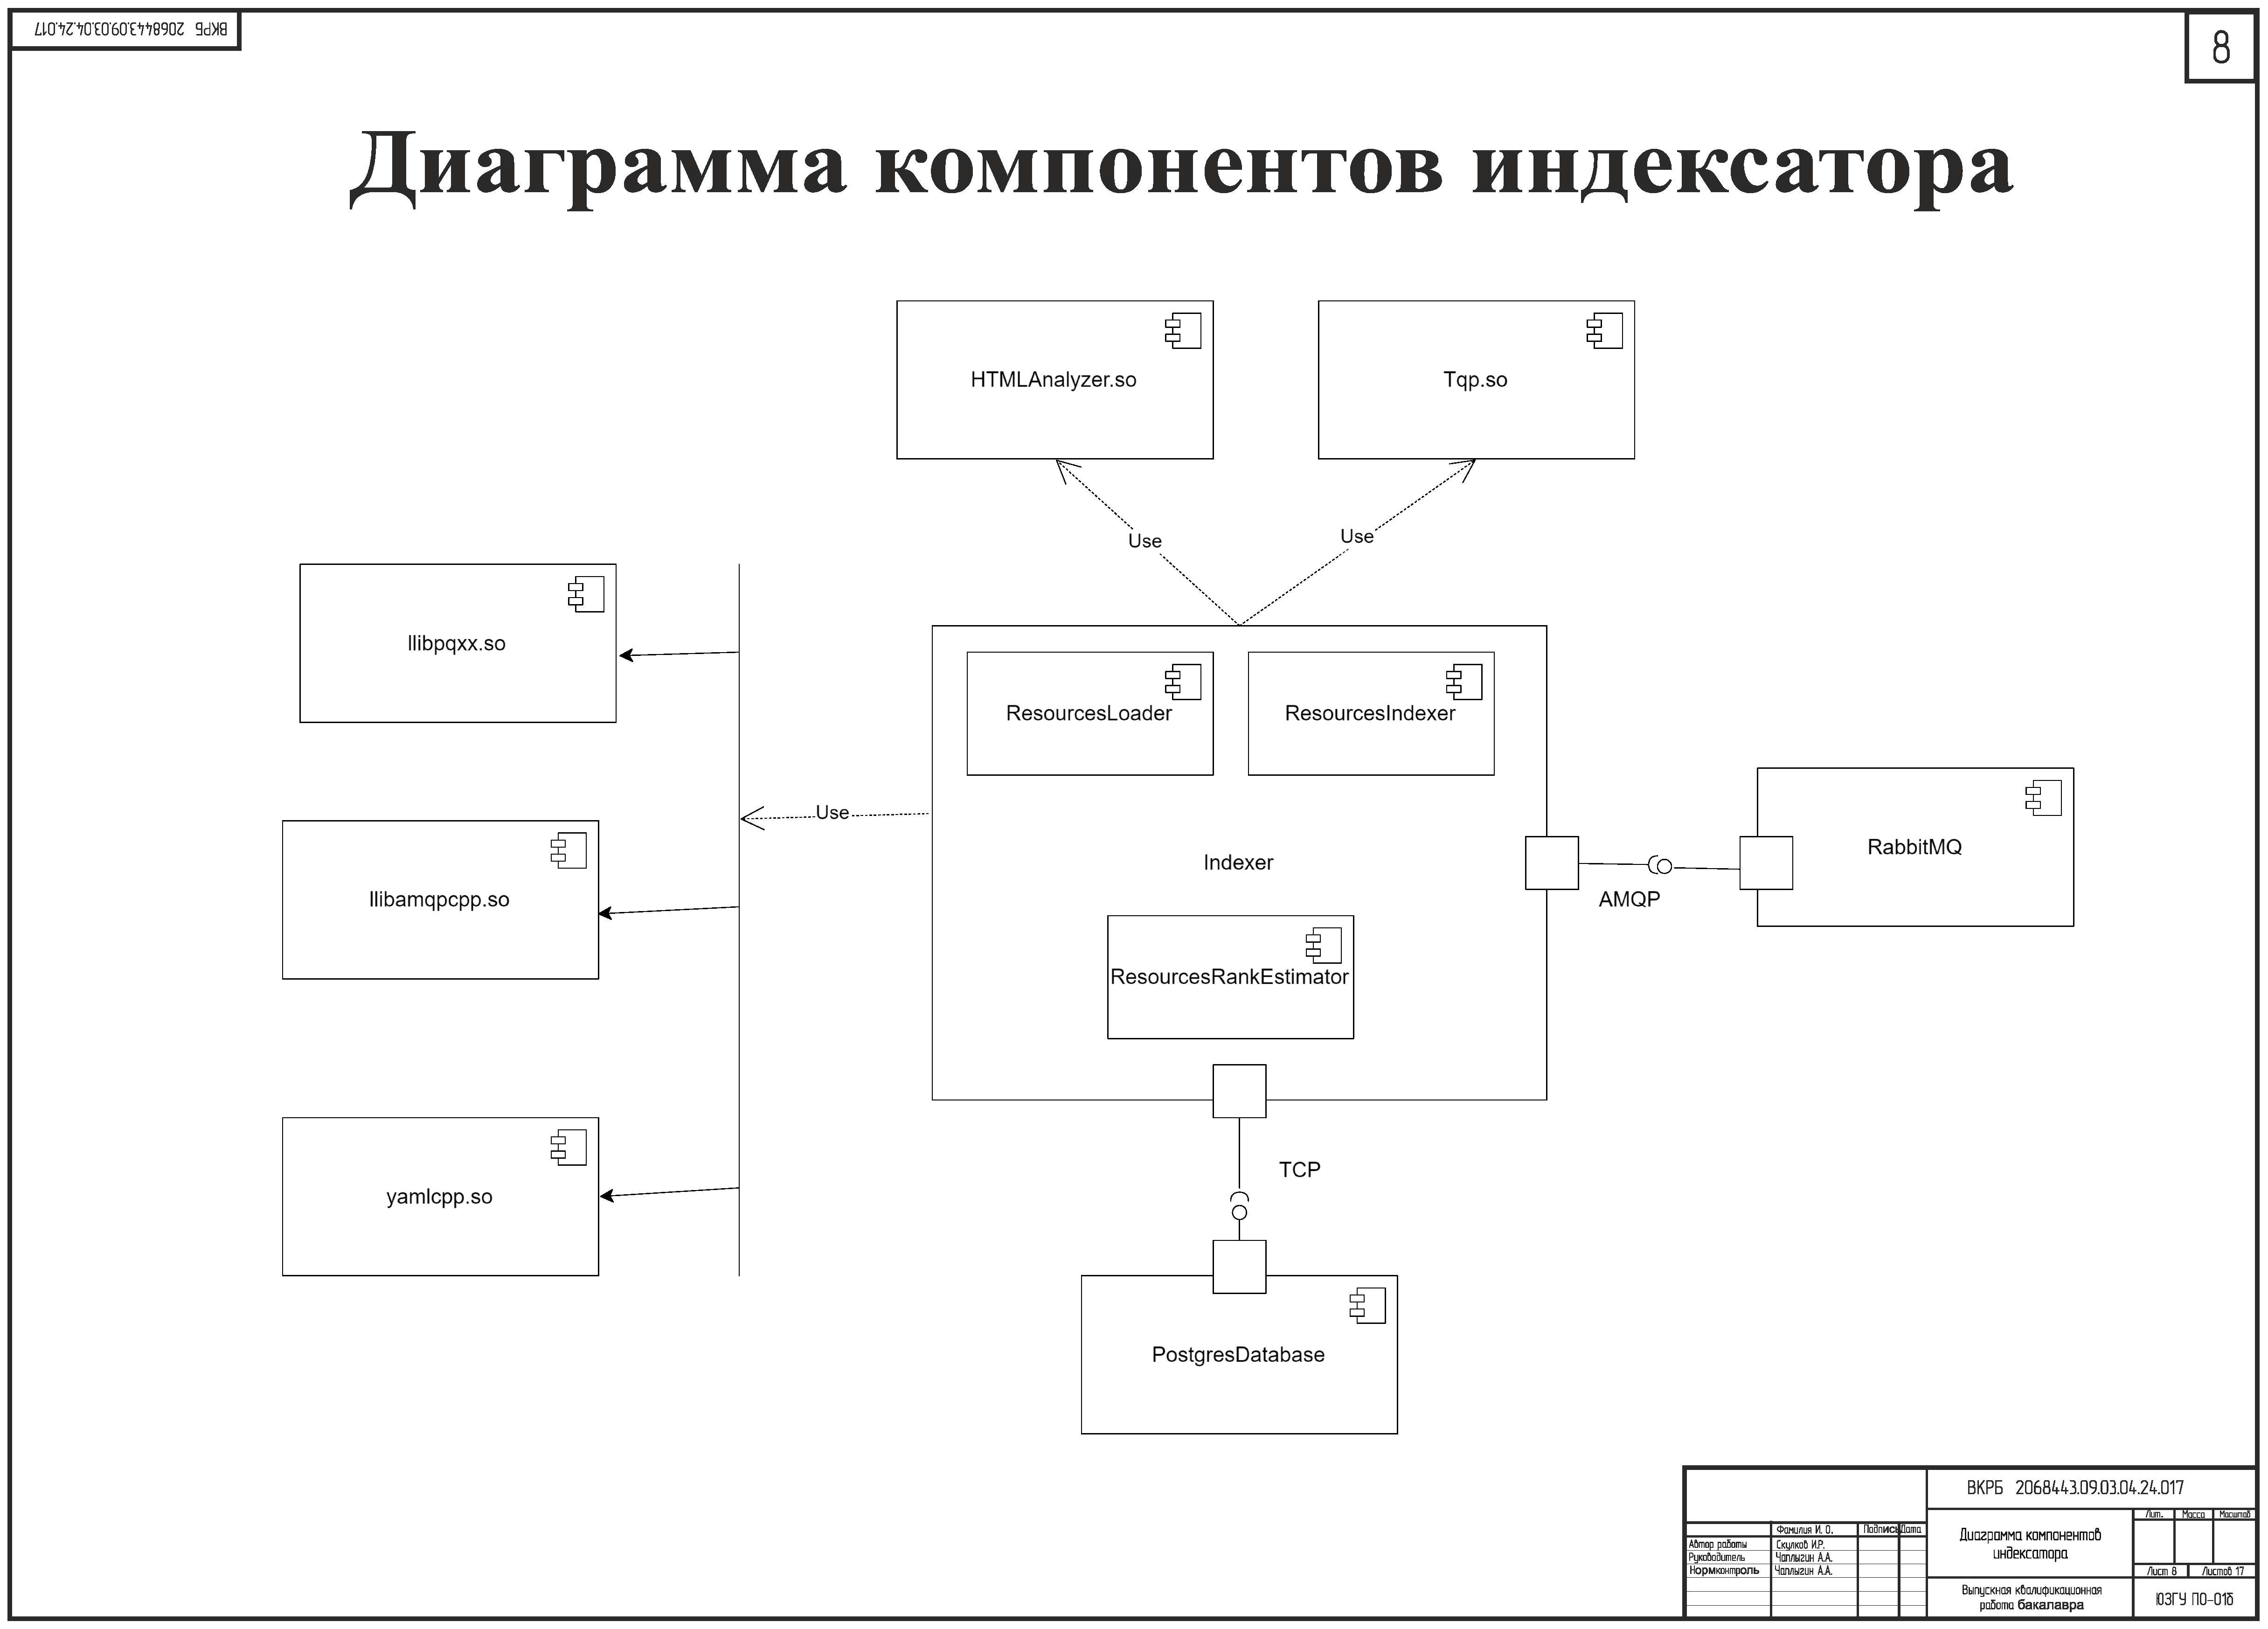
\includegraphics[width=0.82\linewidth]{posters/pi1.eps}
    \заголовок{Диаграмма компонентов индексатора}
    \label{pi1:image}      
\end{плакат}

\begin{плакат}
    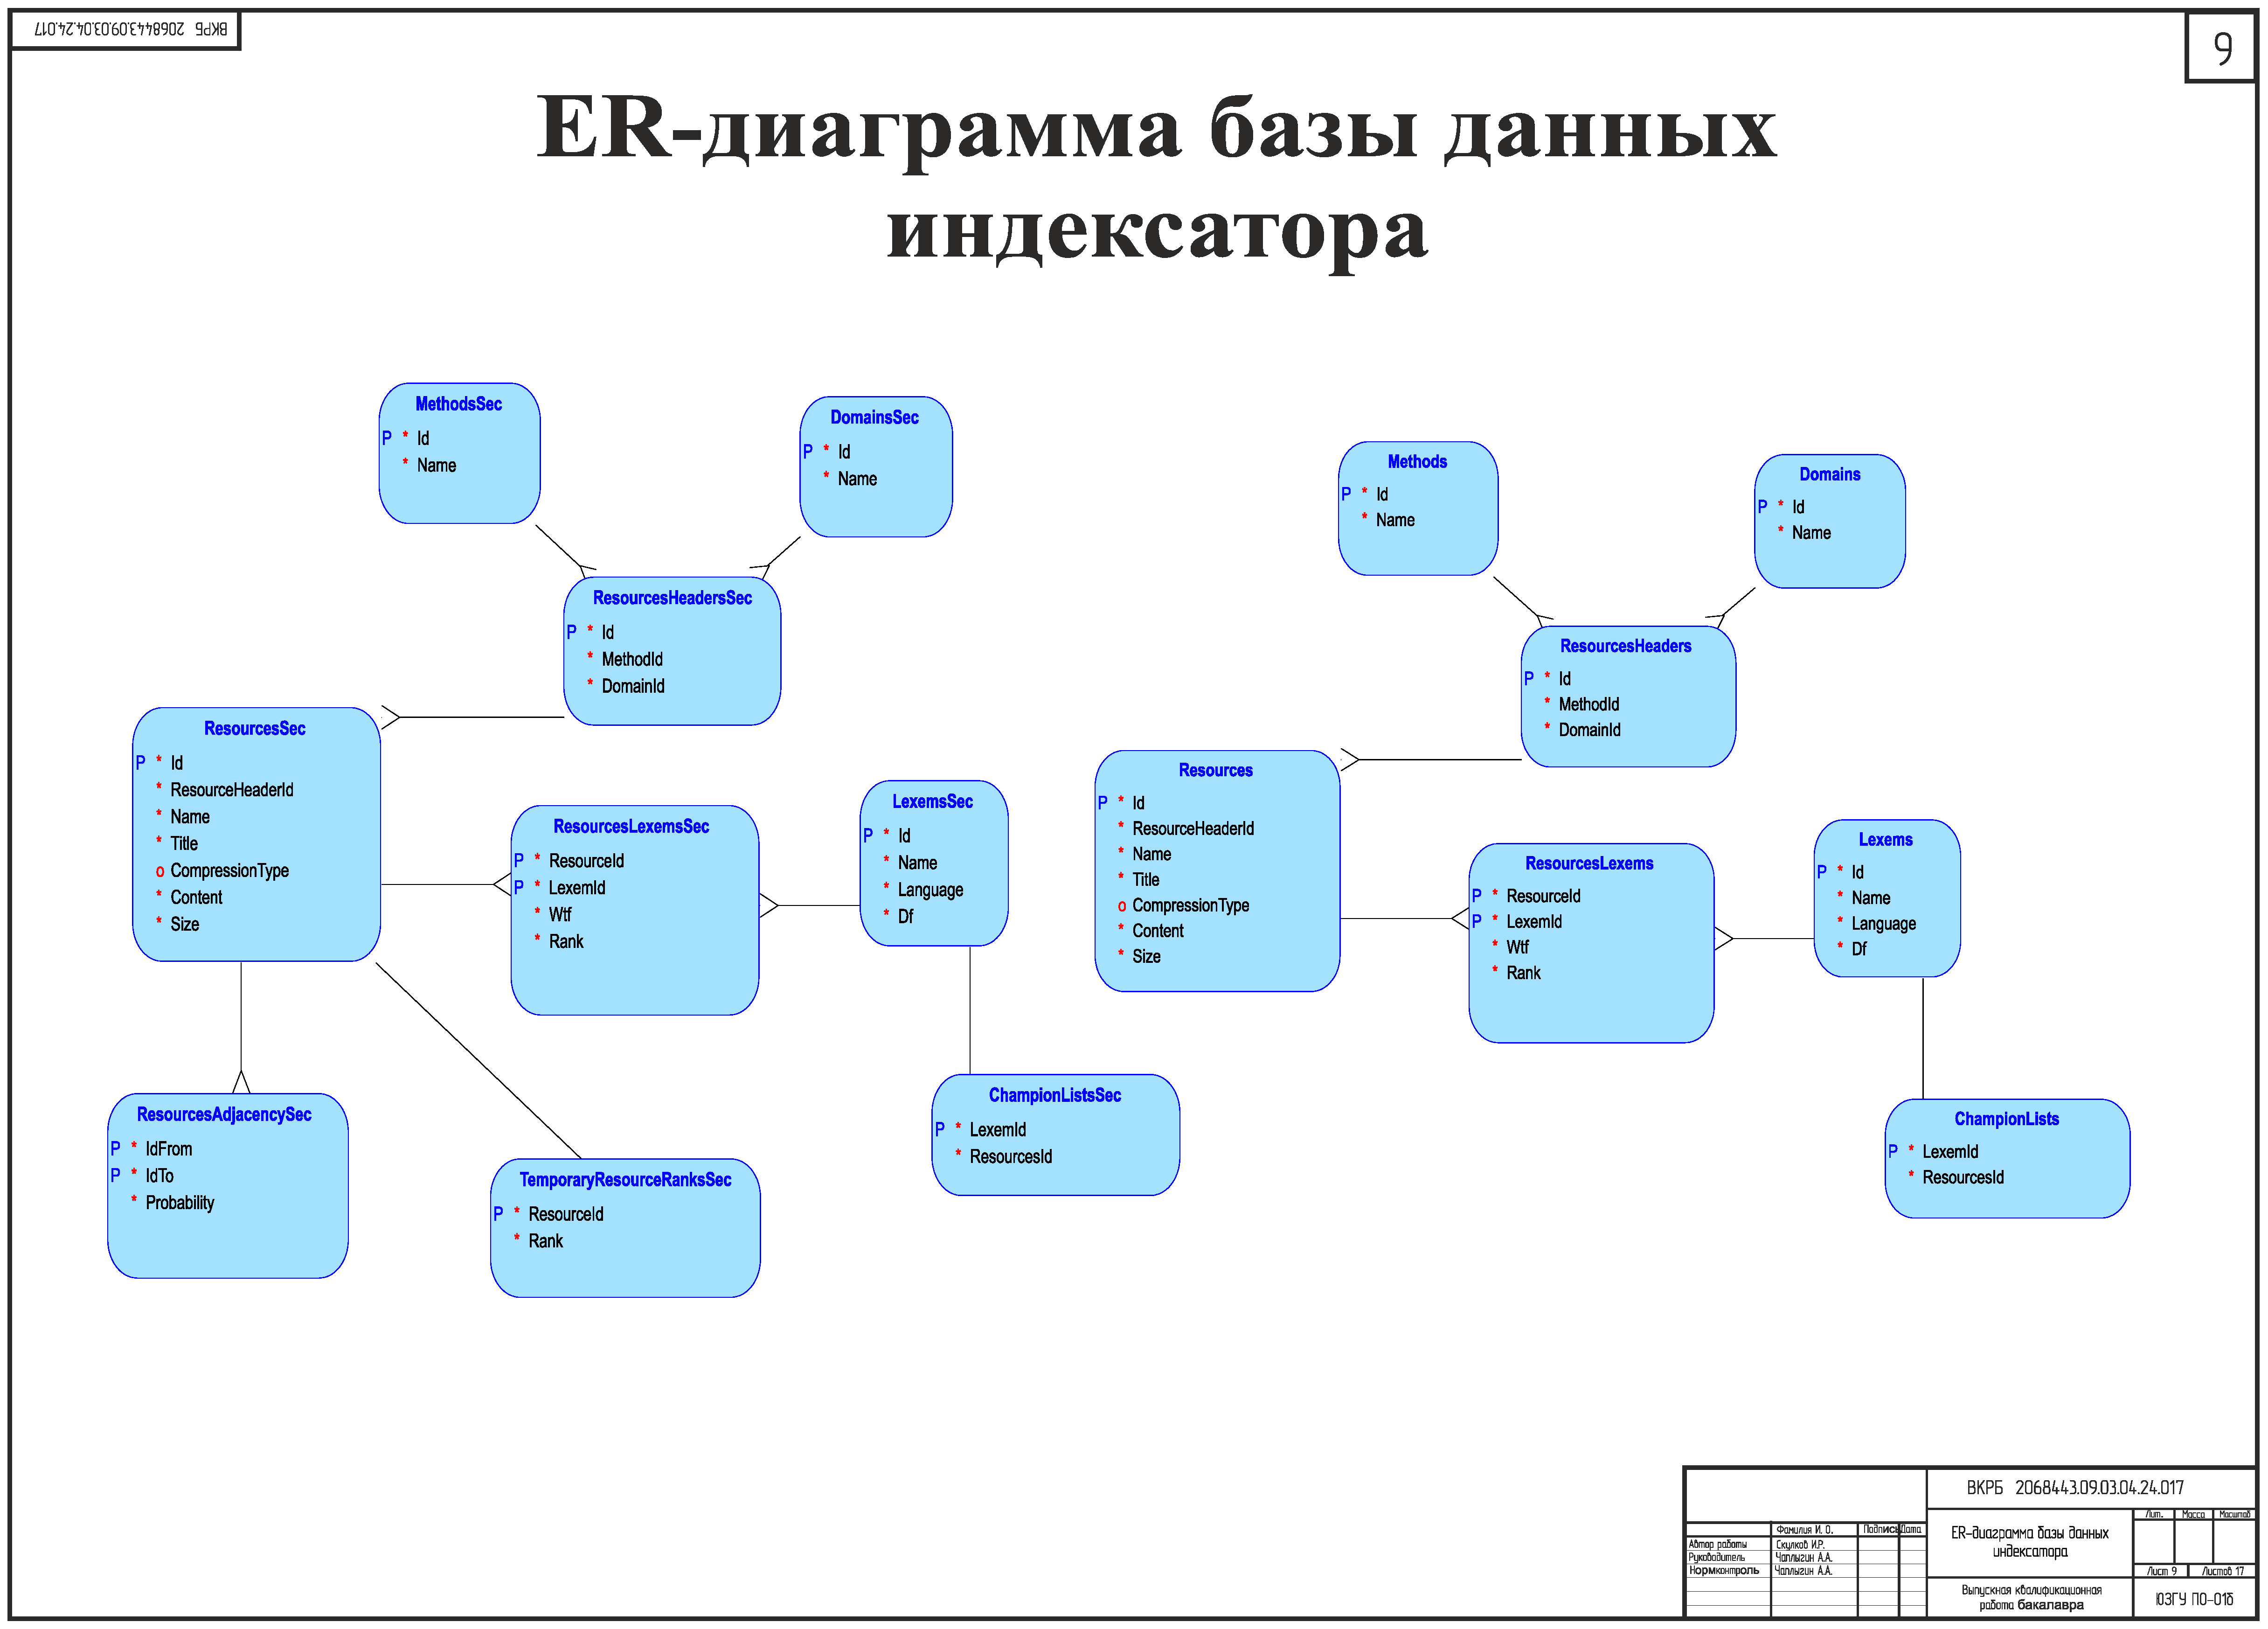
\includegraphics[width=0.82\linewidth]{posters/pi2.eps}
    \заголовок{ER-диаграмма базы данных индексатора}
    \label{pi2:image}      
\end{плакат}

\begin{плакат}
    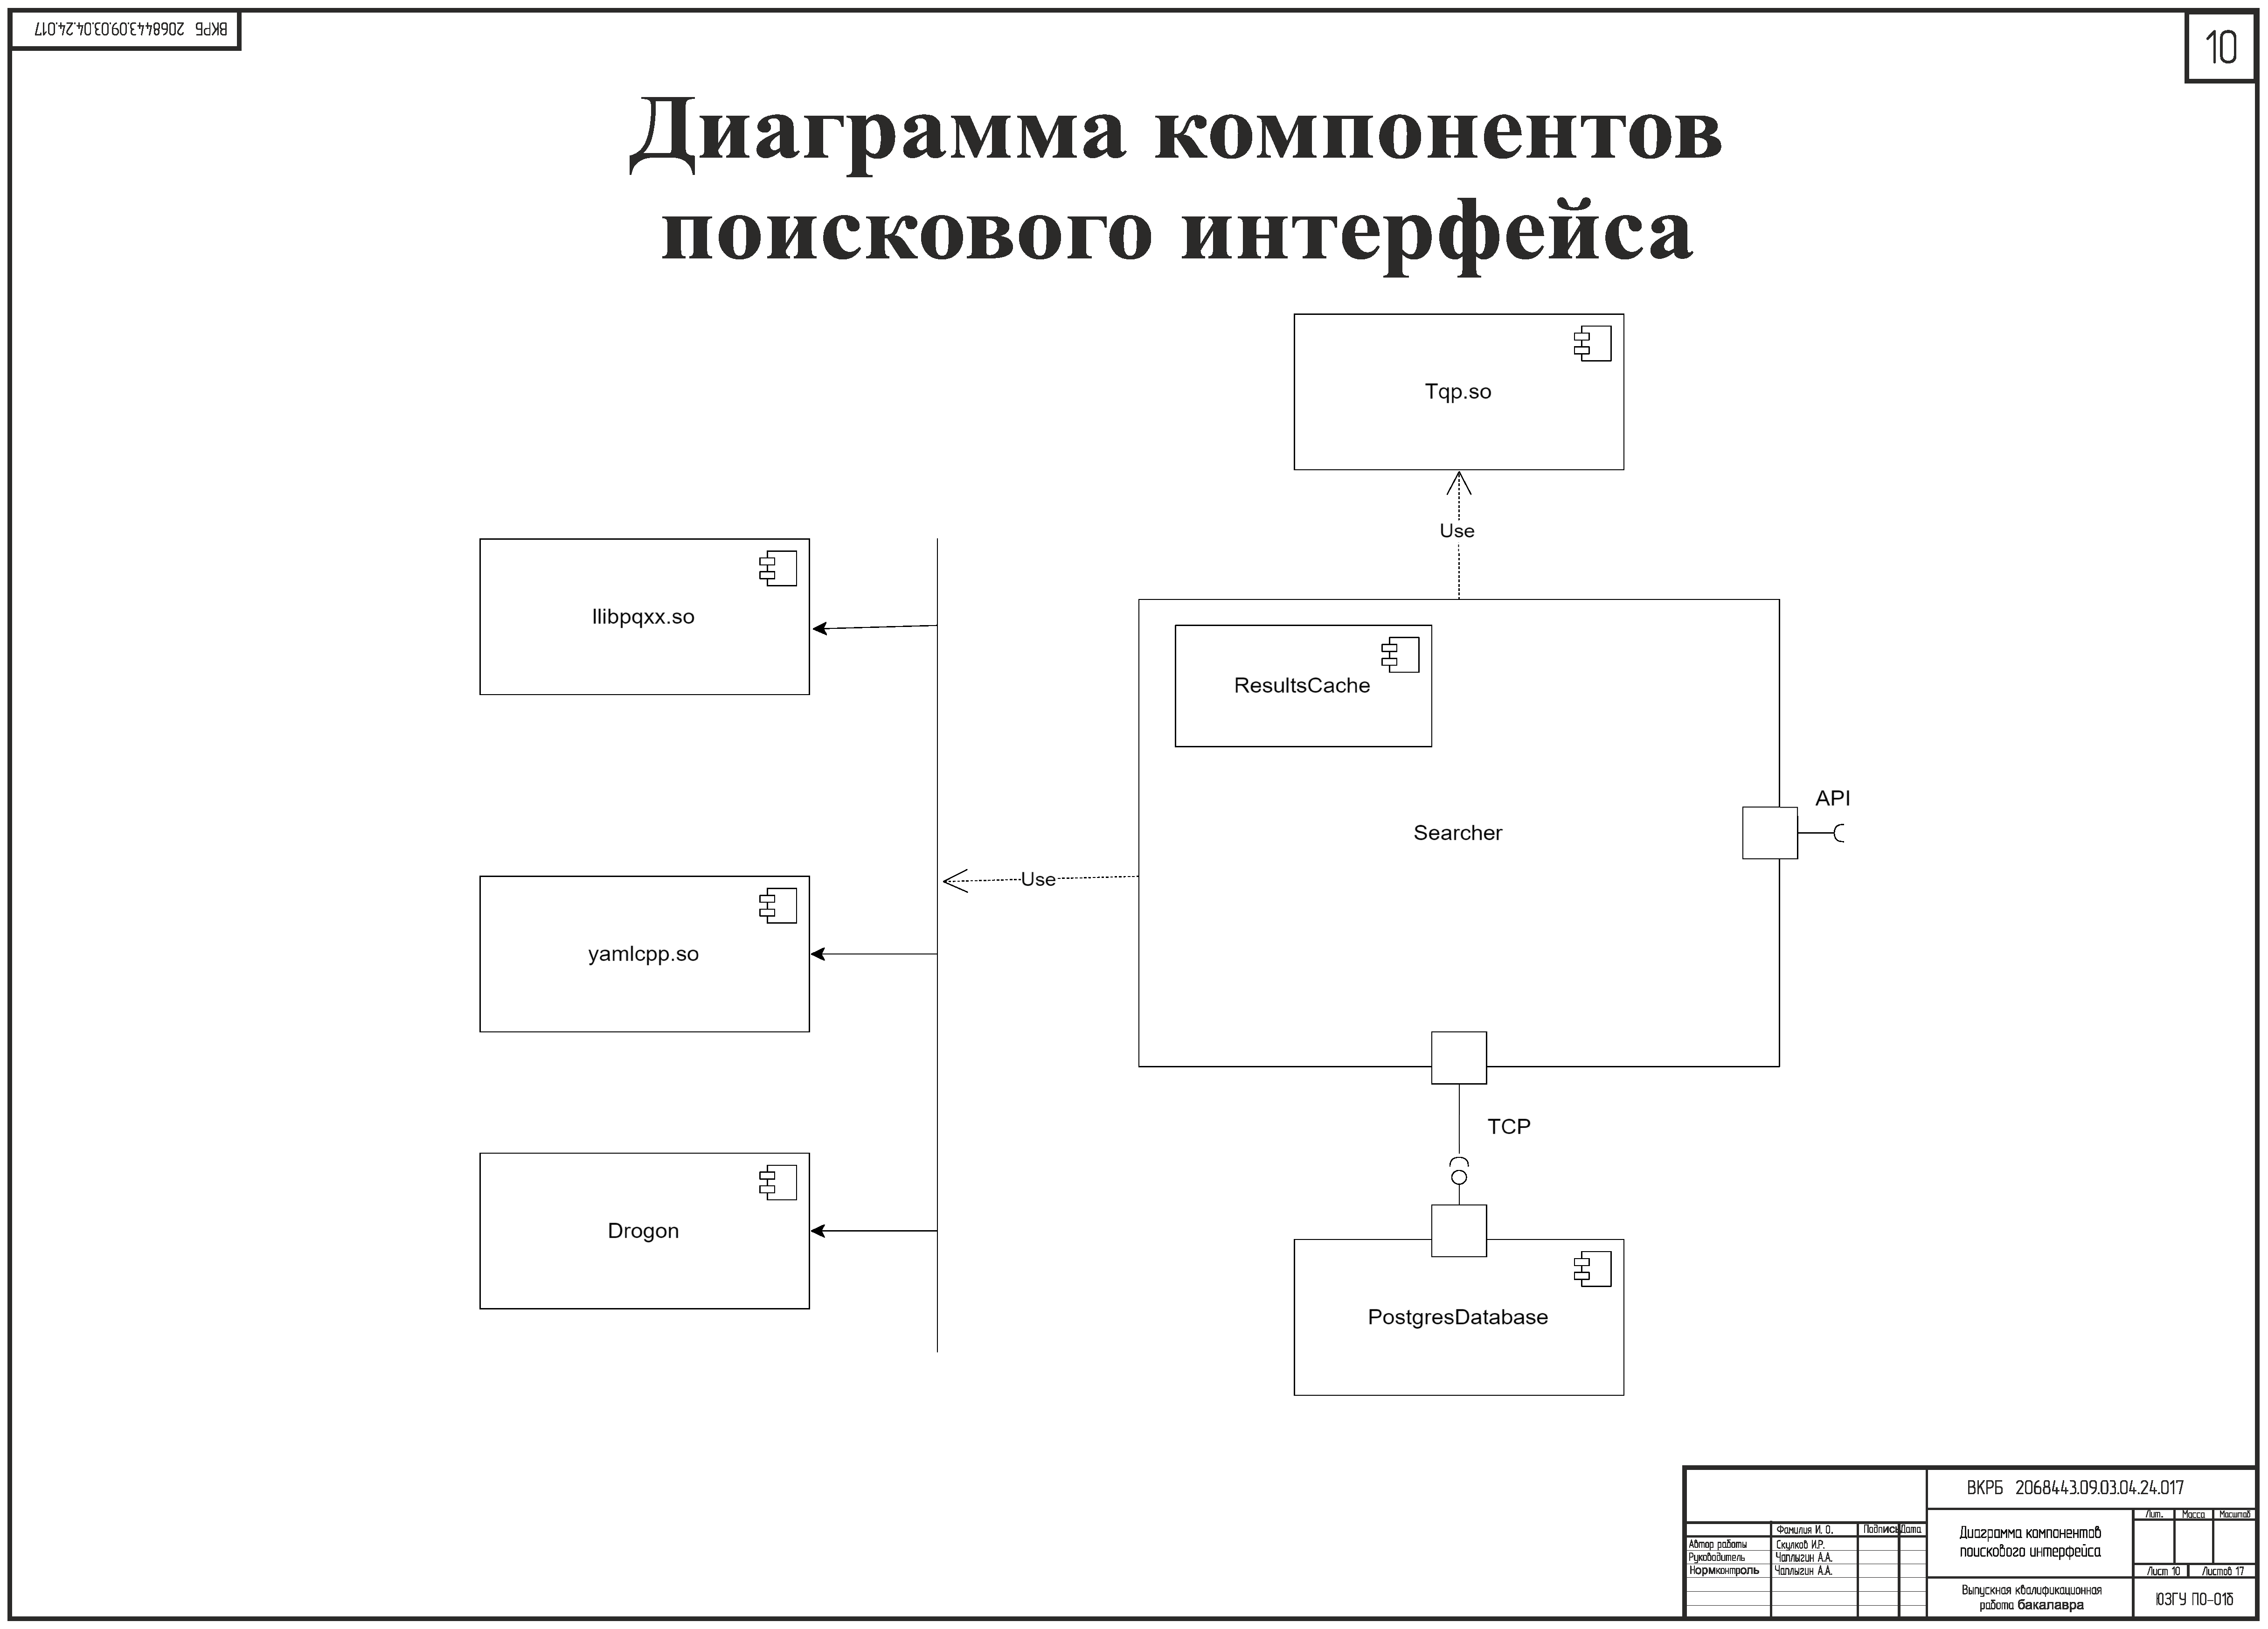
\includegraphics[width=0.82\linewidth]{posters/ps1.eps}
    \заголовок{Диаграмма компонентов поискового интерфейса}
    \label{ps1:image}      
\end{плакат}

\begin{плакат}
    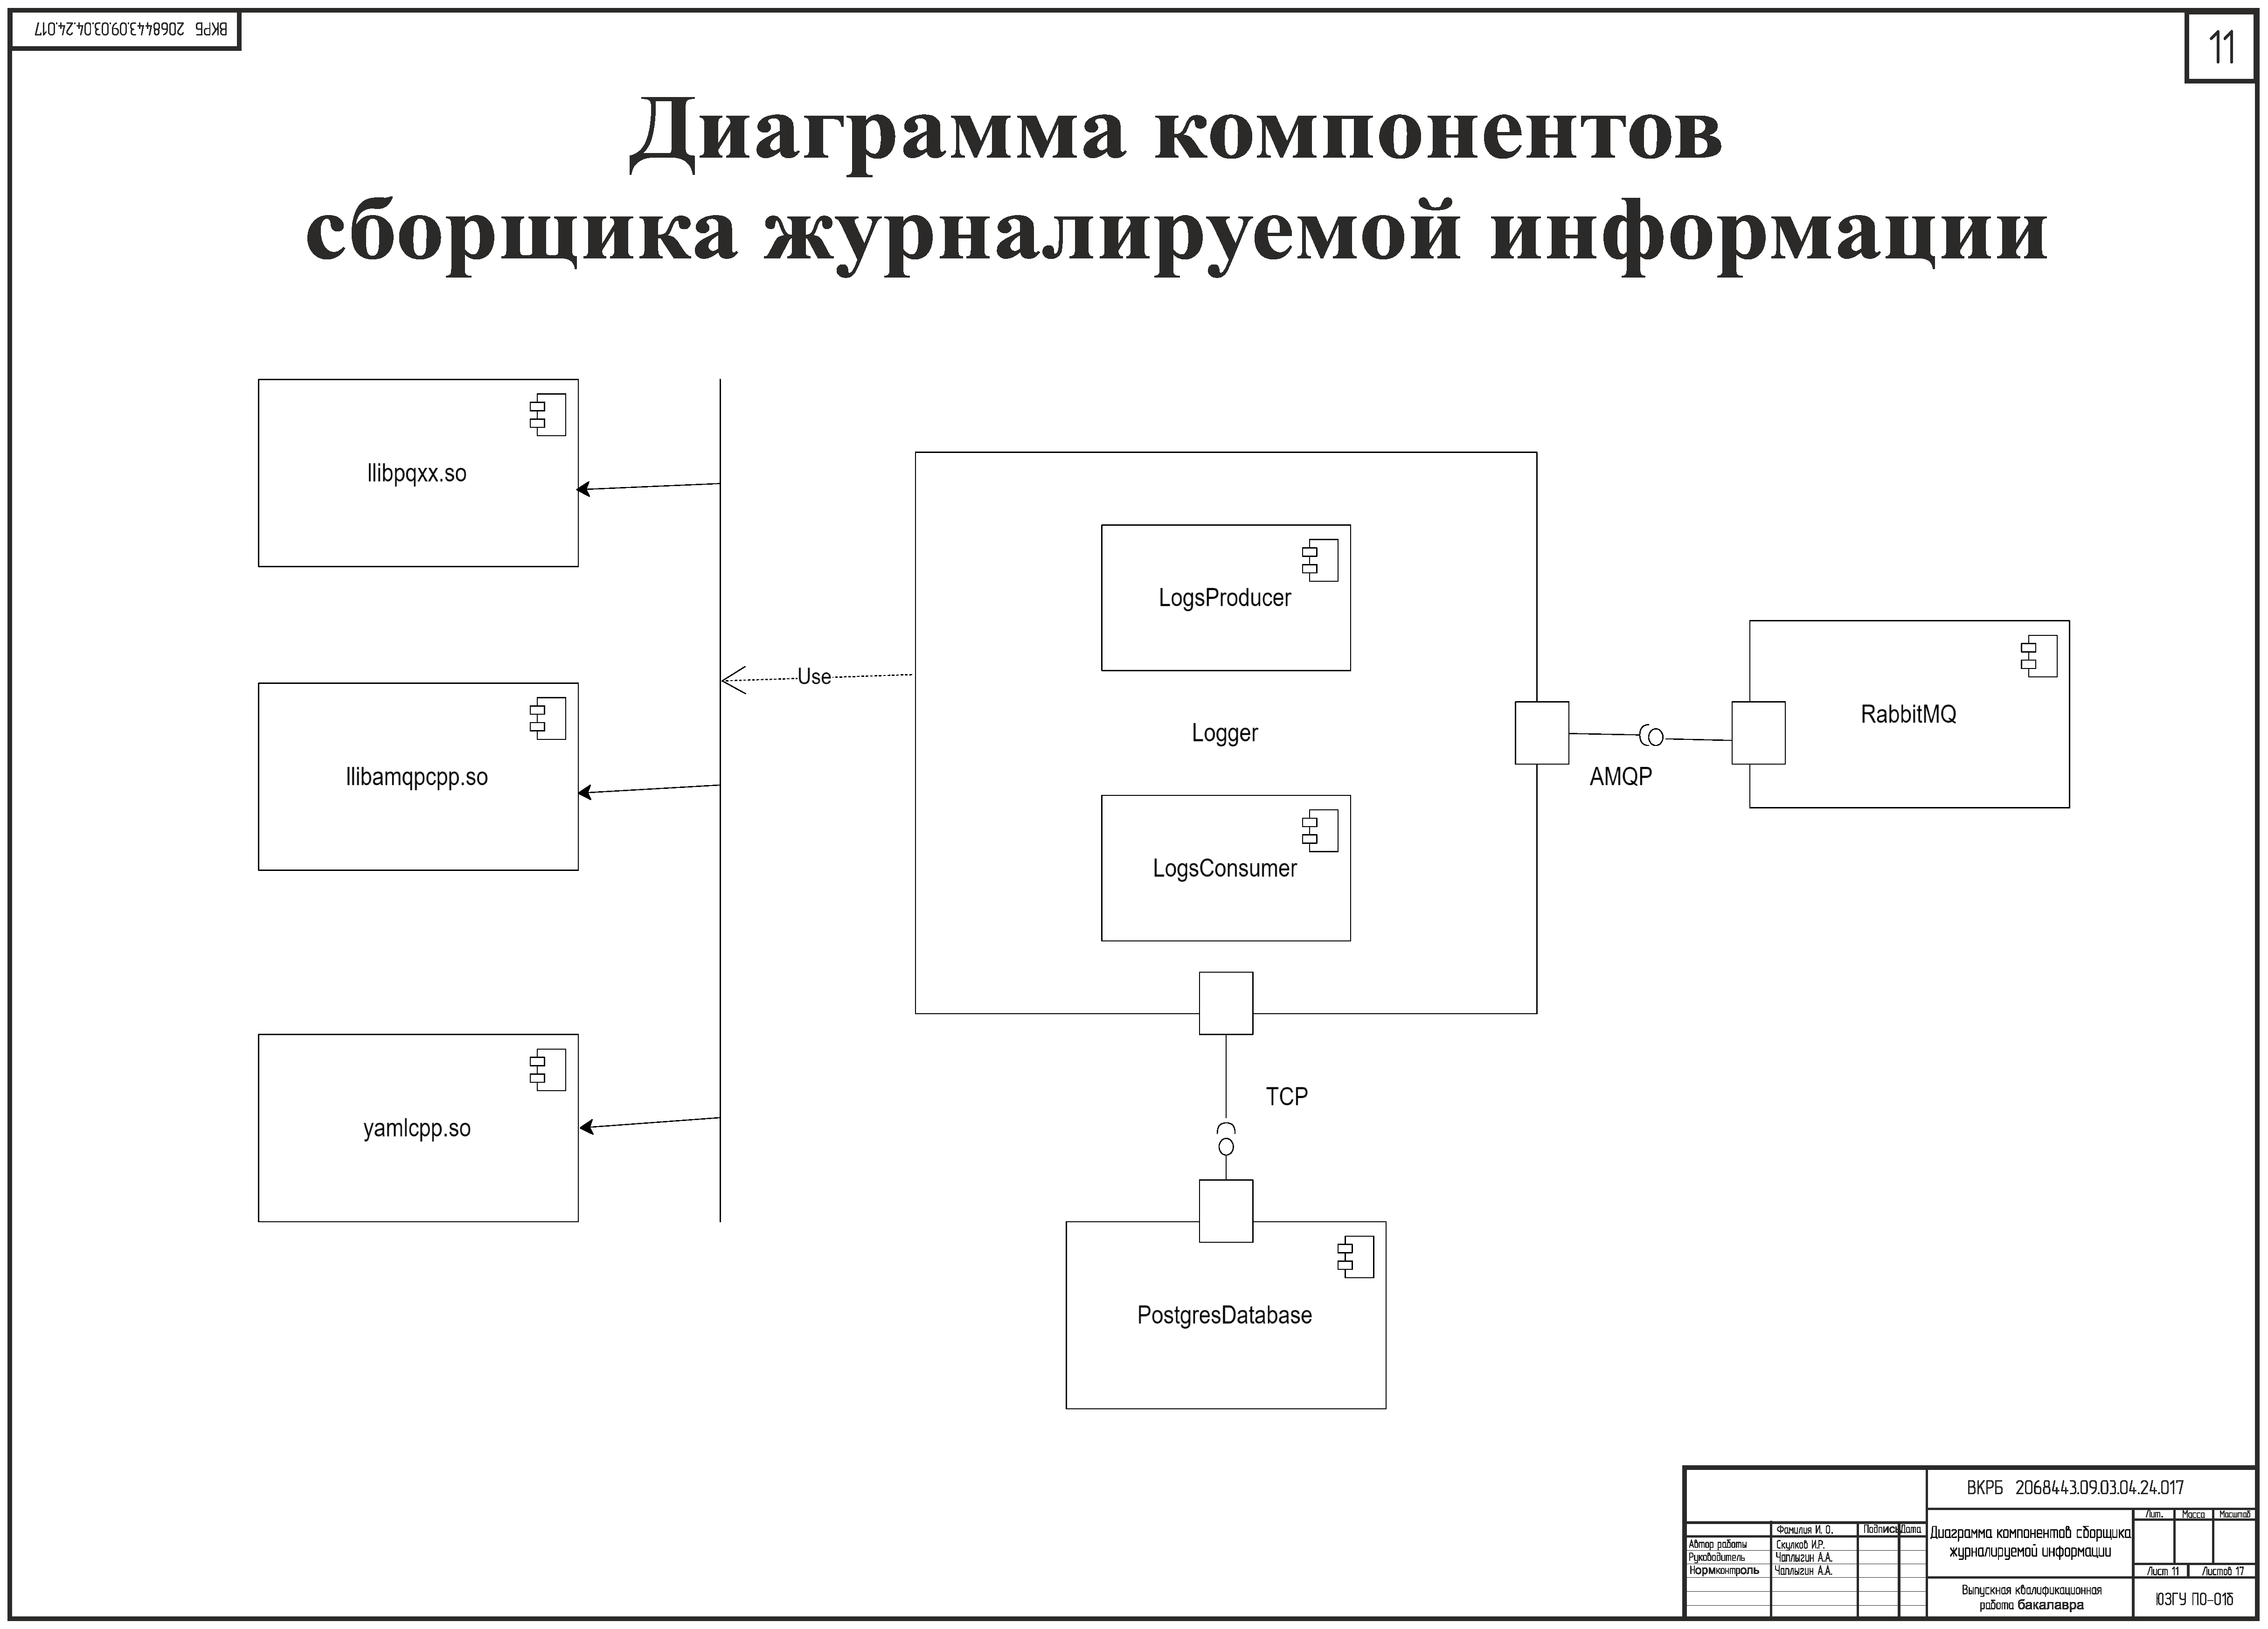
\includegraphics[width=0.82\linewidth]{posters/pl1.eps}
    \заголовок{Диаграмма компонентов сборщика журналируемой информации}
    \label{pl1:image}      
\end{плакат}

\begin{плакат}
    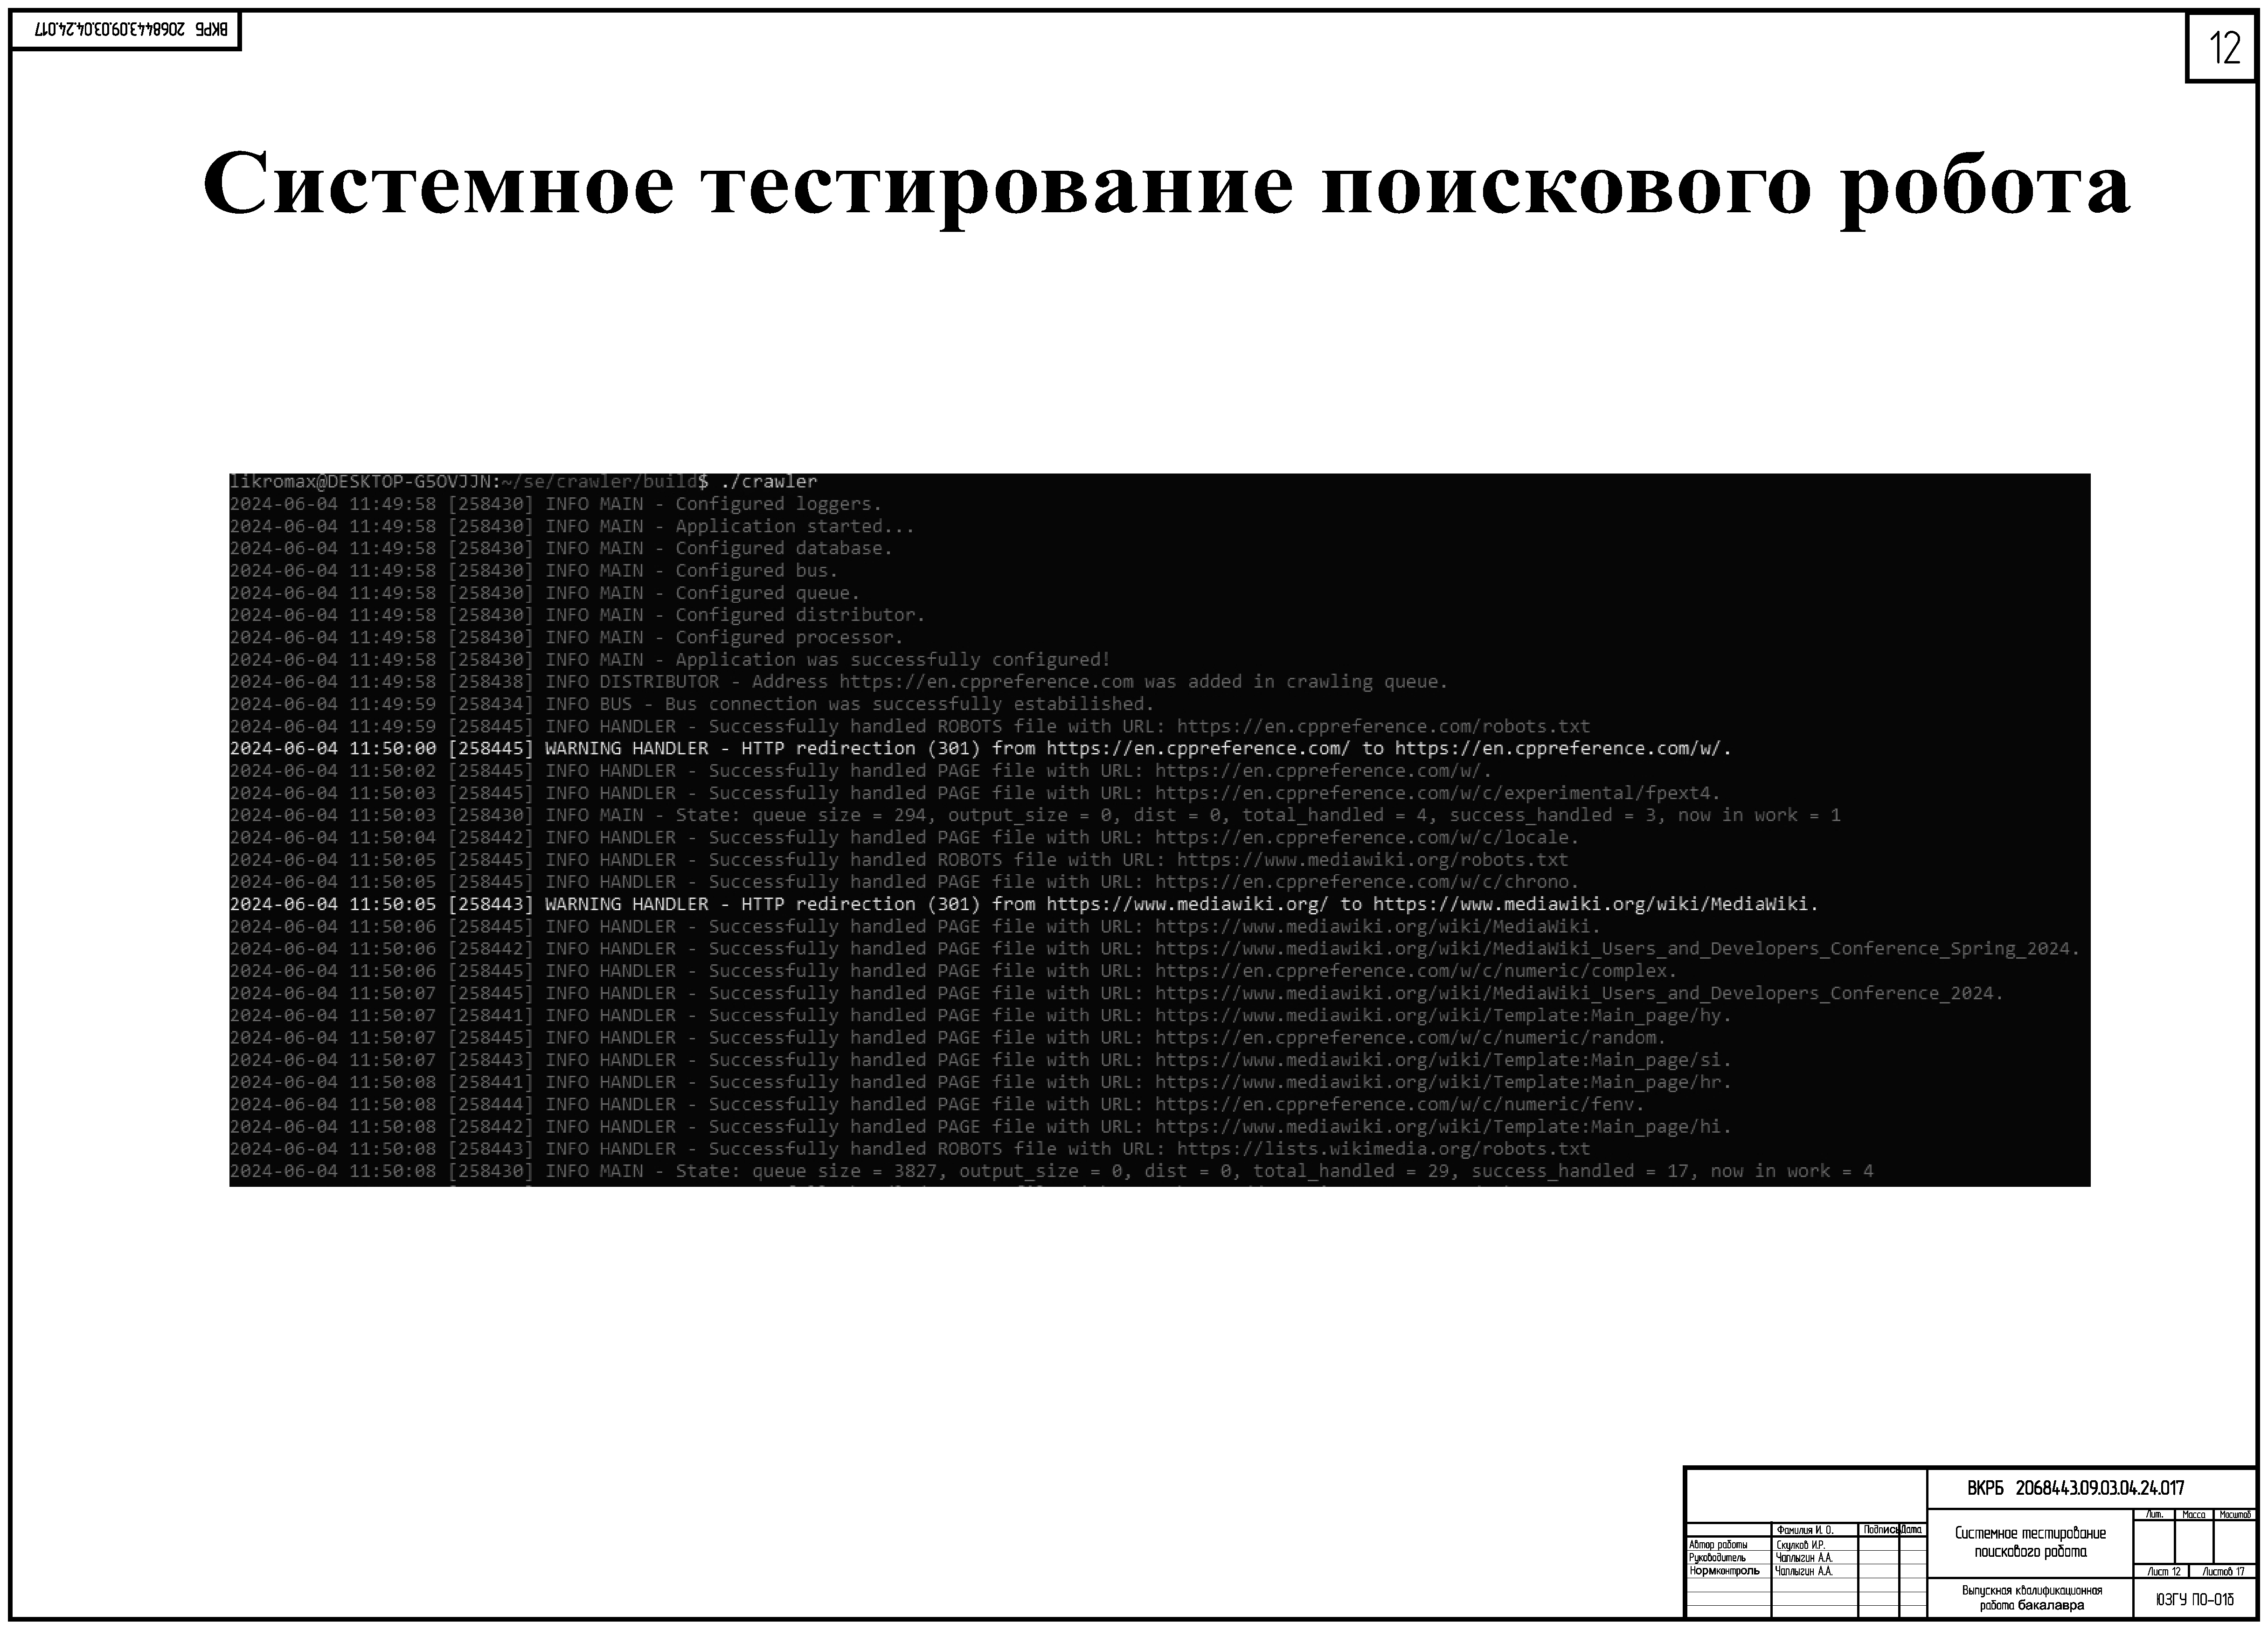
\includegraphics[width=0.82\linewidth]{posters/ptr.eps}
    \заголовок{Системное тестирование поискового робота}
    \label{ptr:image}      
\end{плакат}

\begin{плакат}
    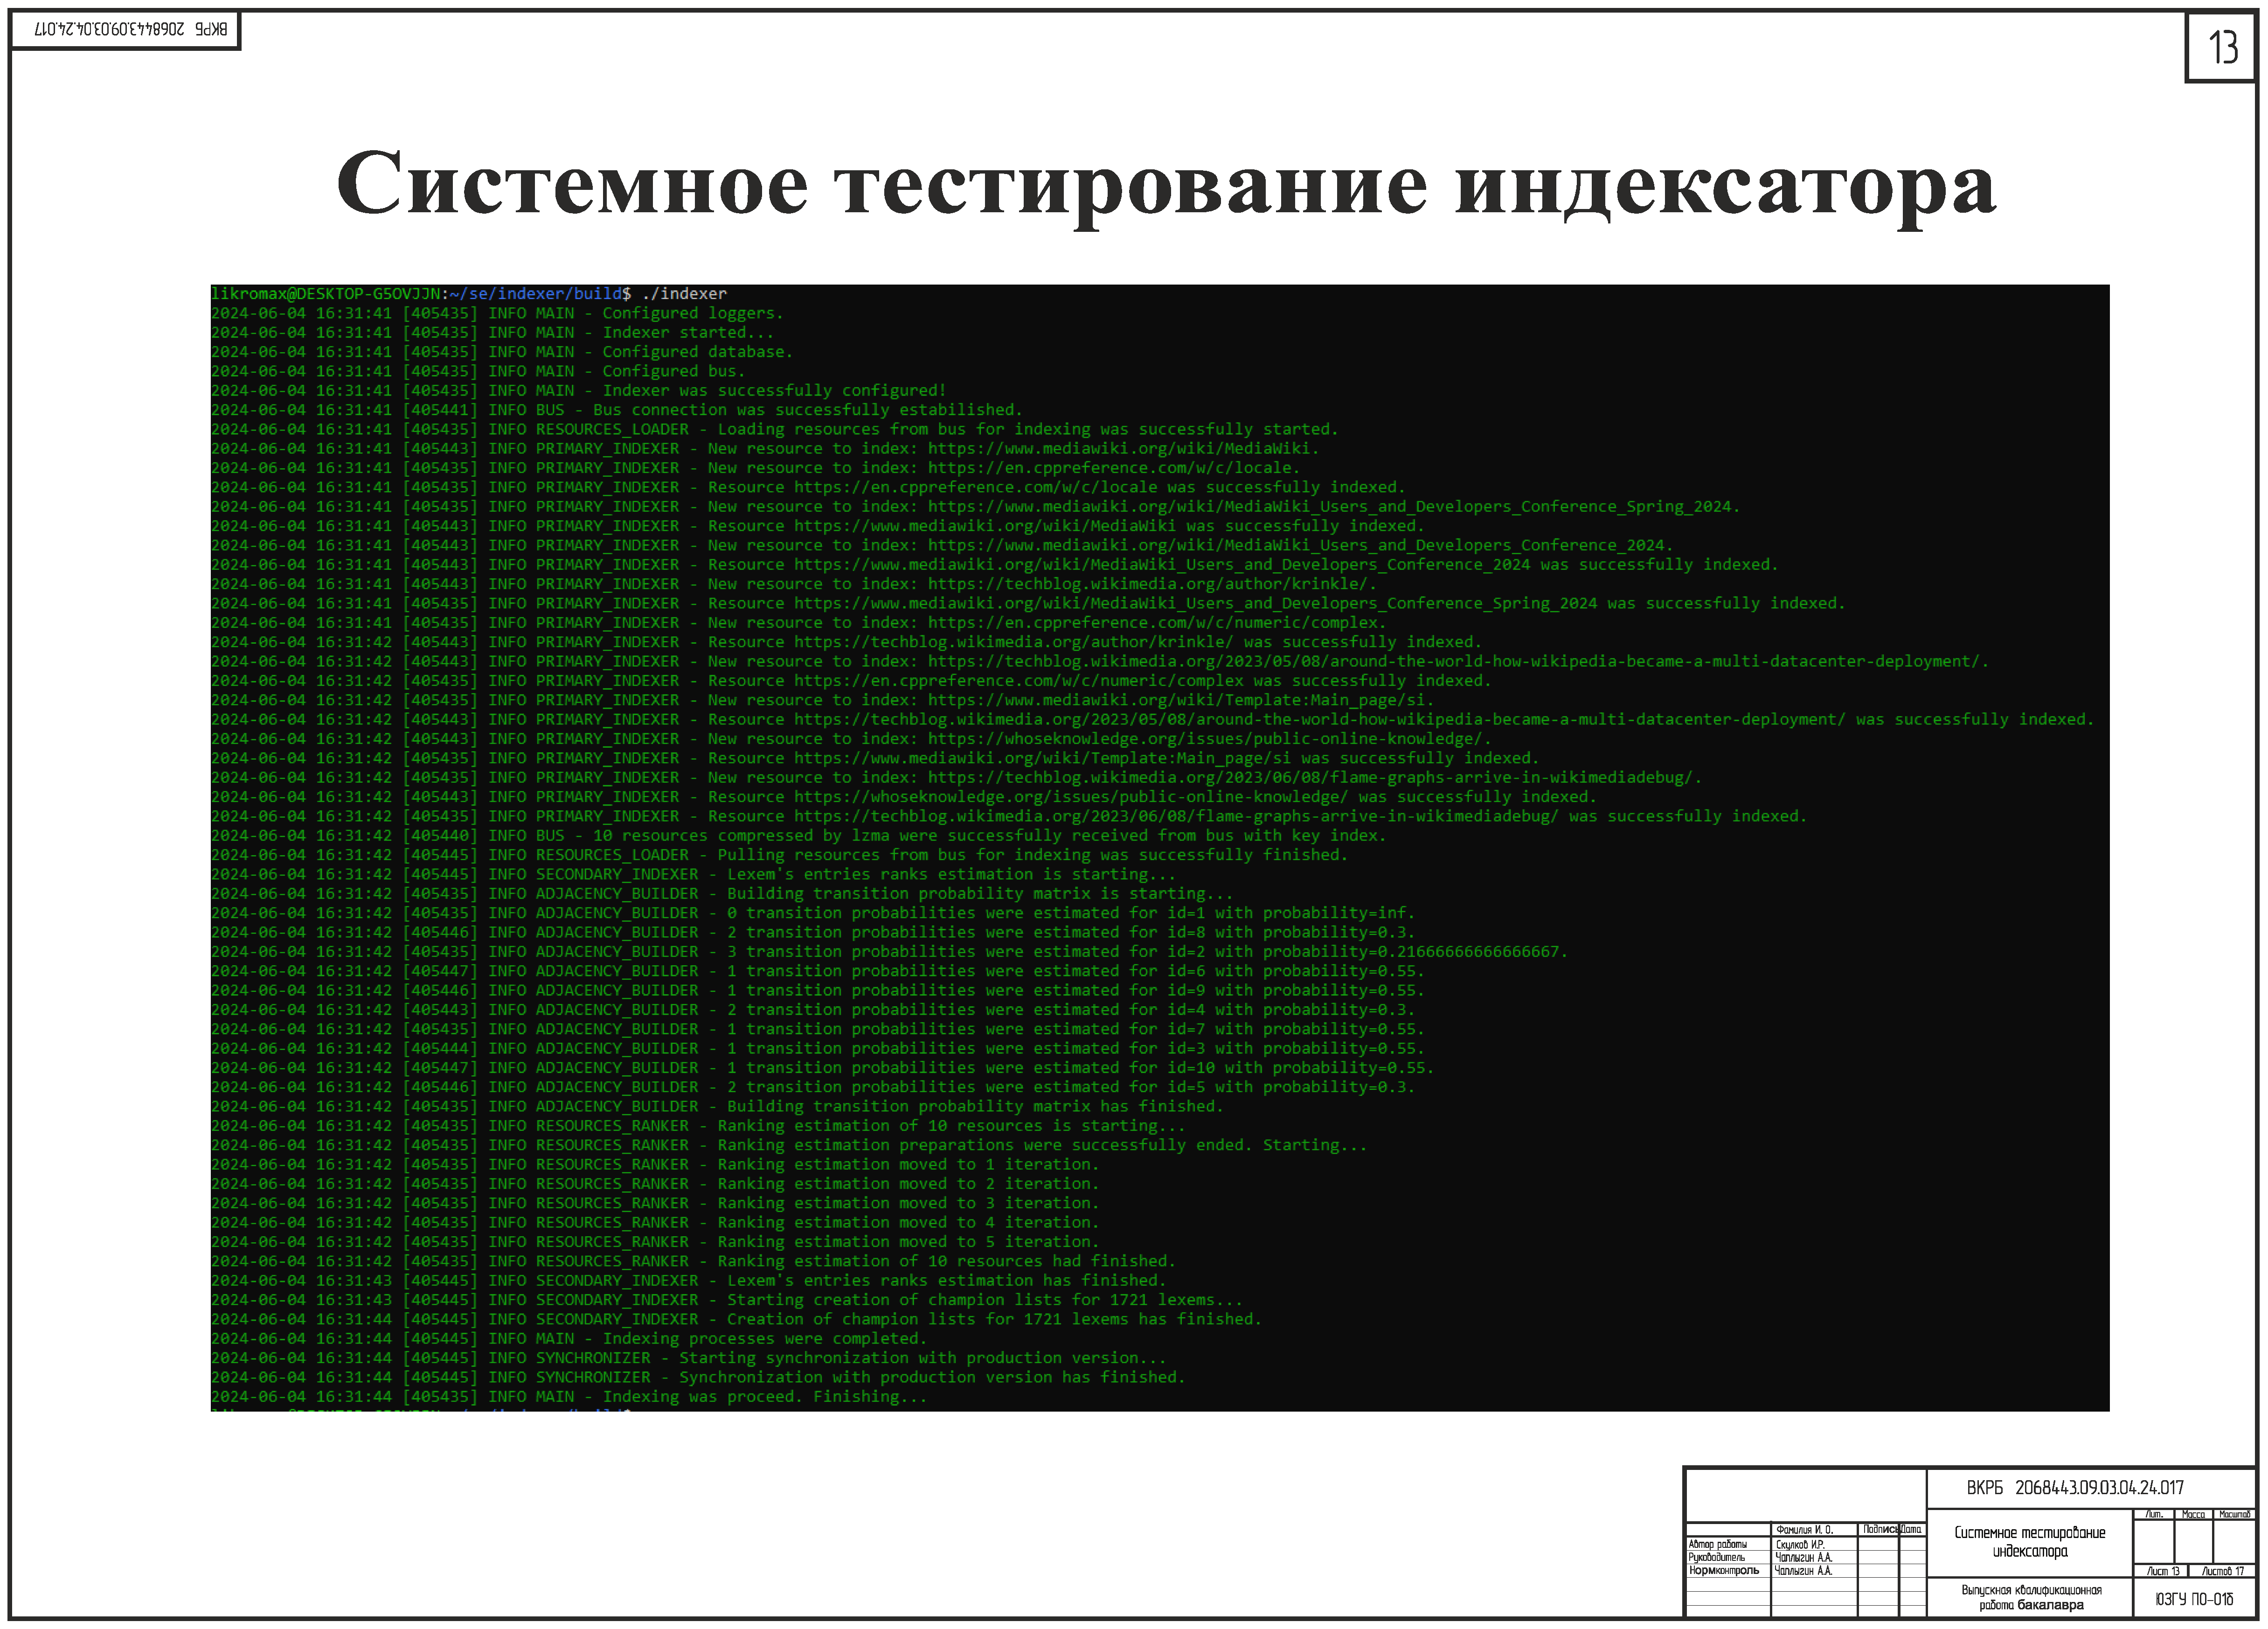
\includegraphics[width=0.82\linewidth]{posters/pti.eps}
    \заголовок{Системное тестирование индексатора}
    \label{pti:image}      
\end{плакат}

\begin{плакат}
    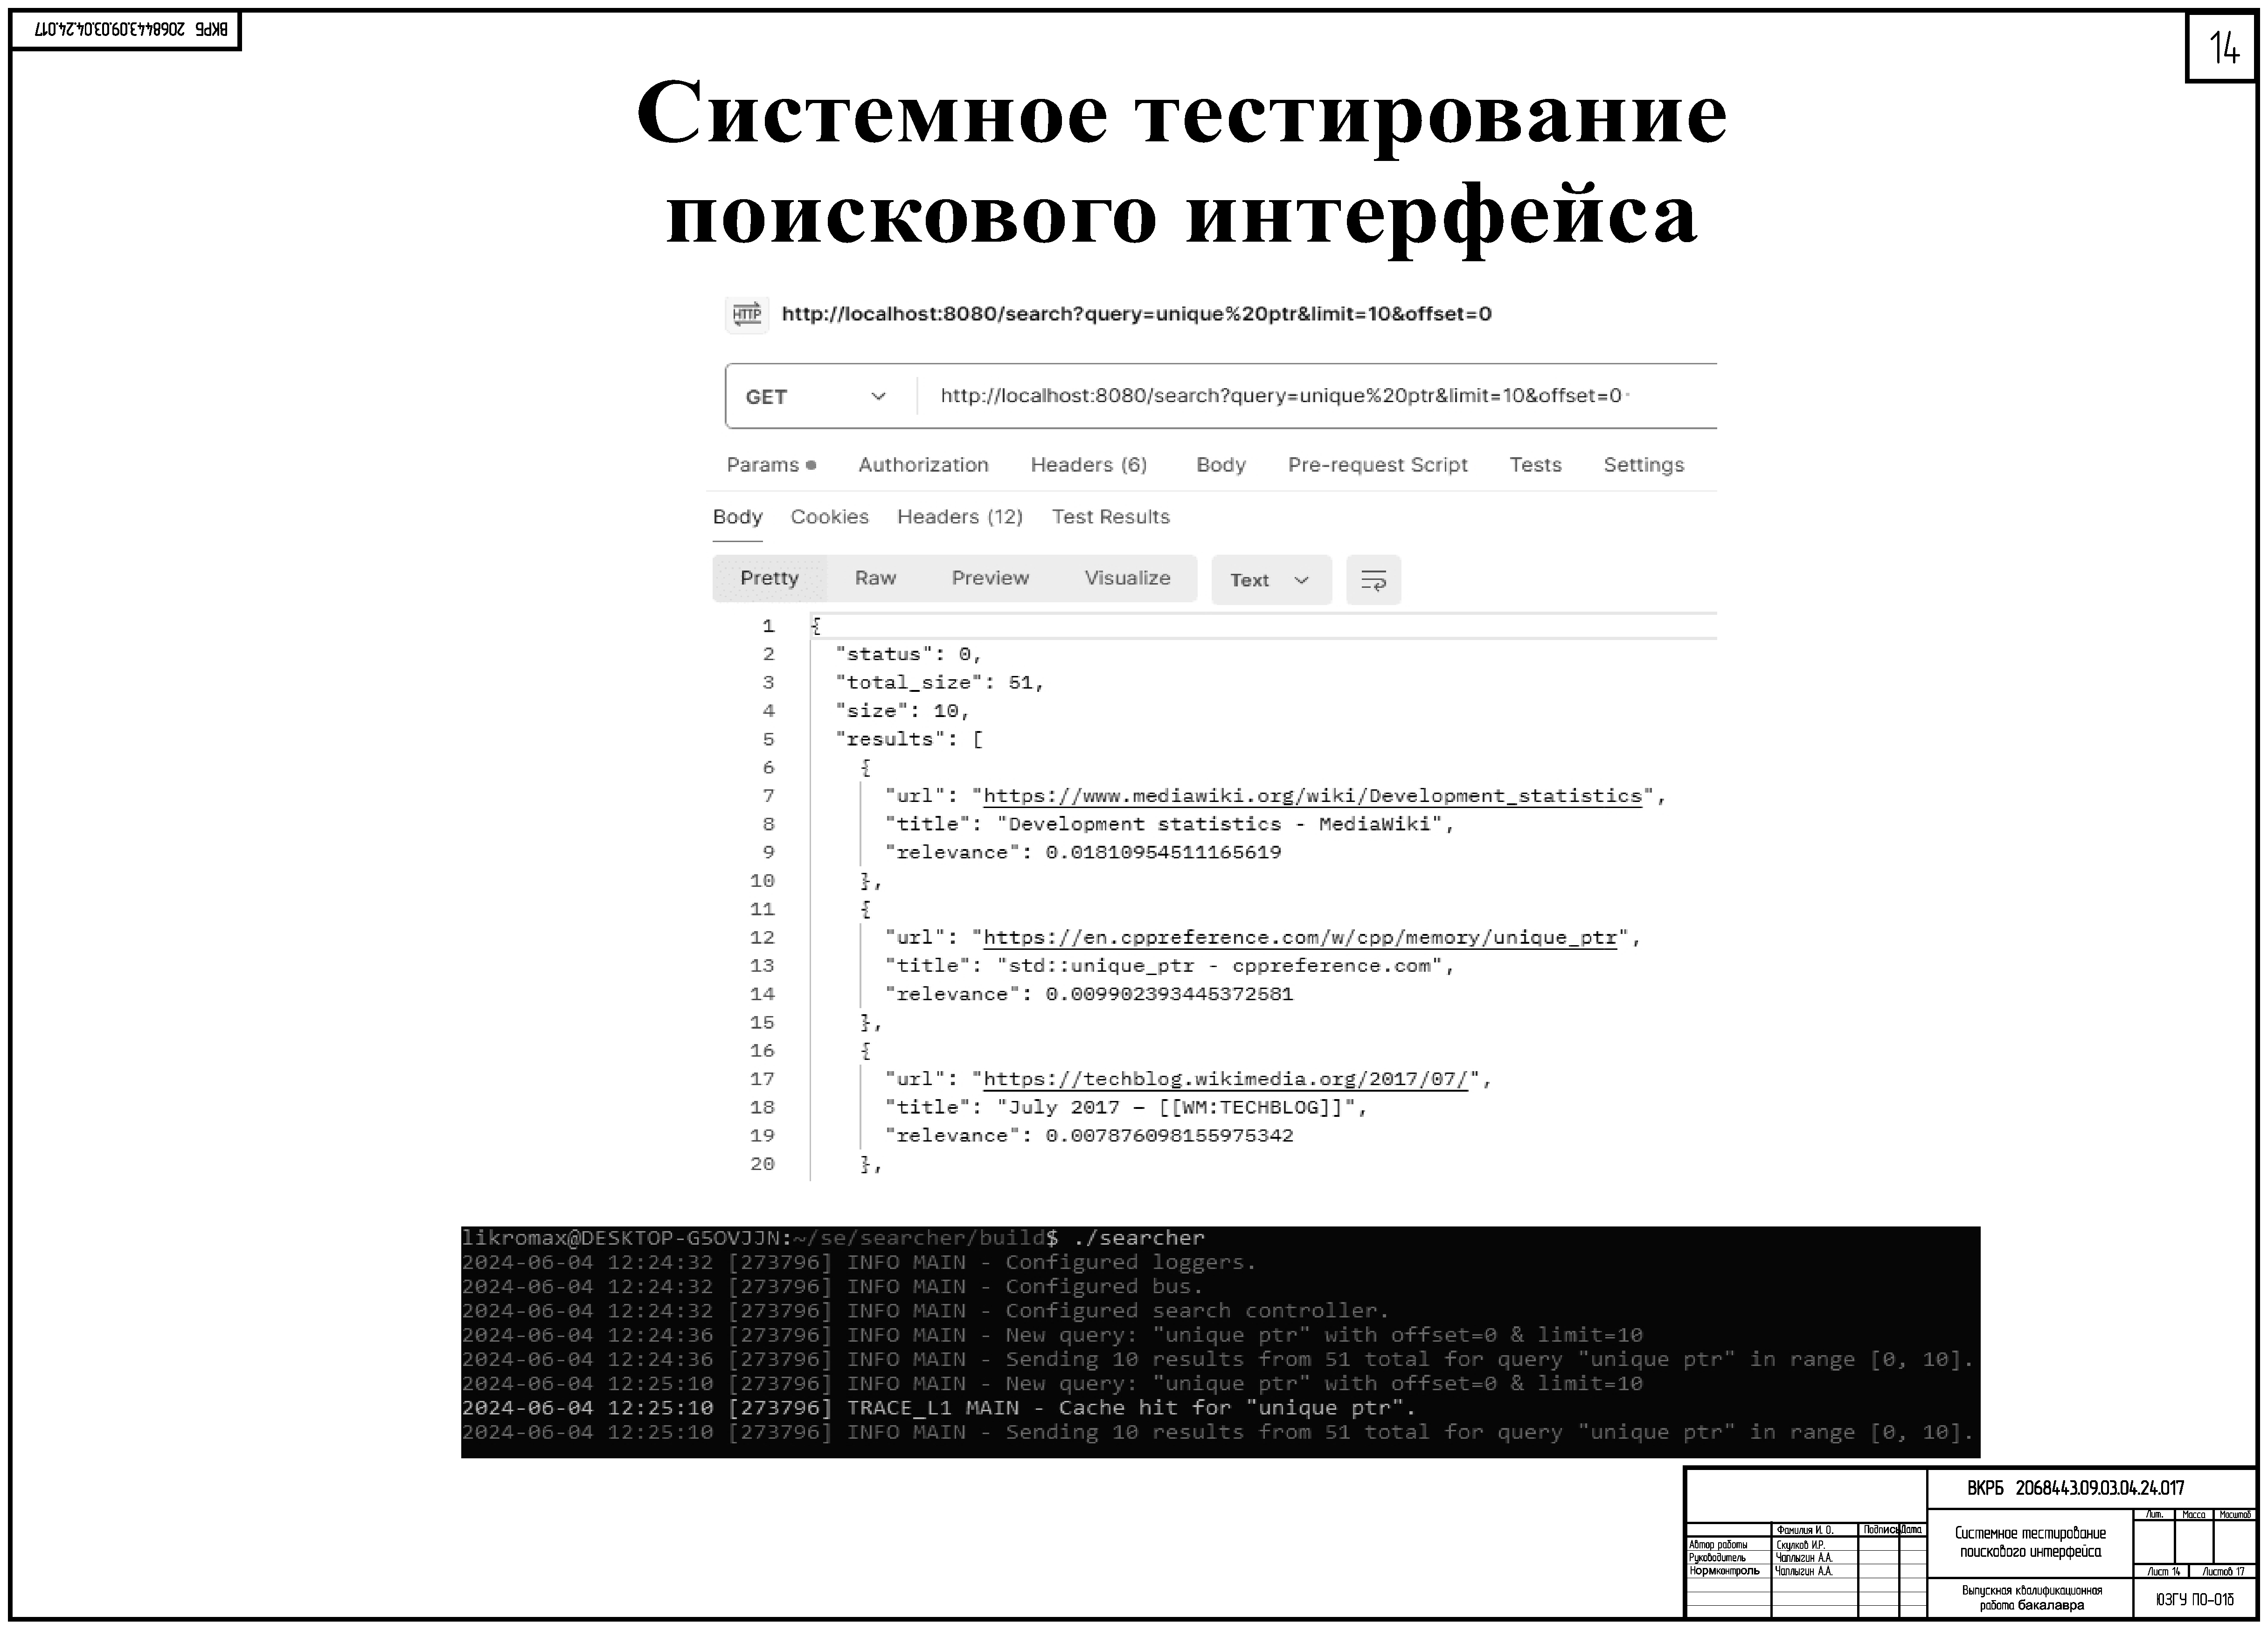
\includegraphics[width=0.82\linewidth]{posters/pts.eps}
    \заголовок{Системное тестирование поискового интерфейса}
    \label{pts:image}      
\end{плакат}

\begin{плакат}
    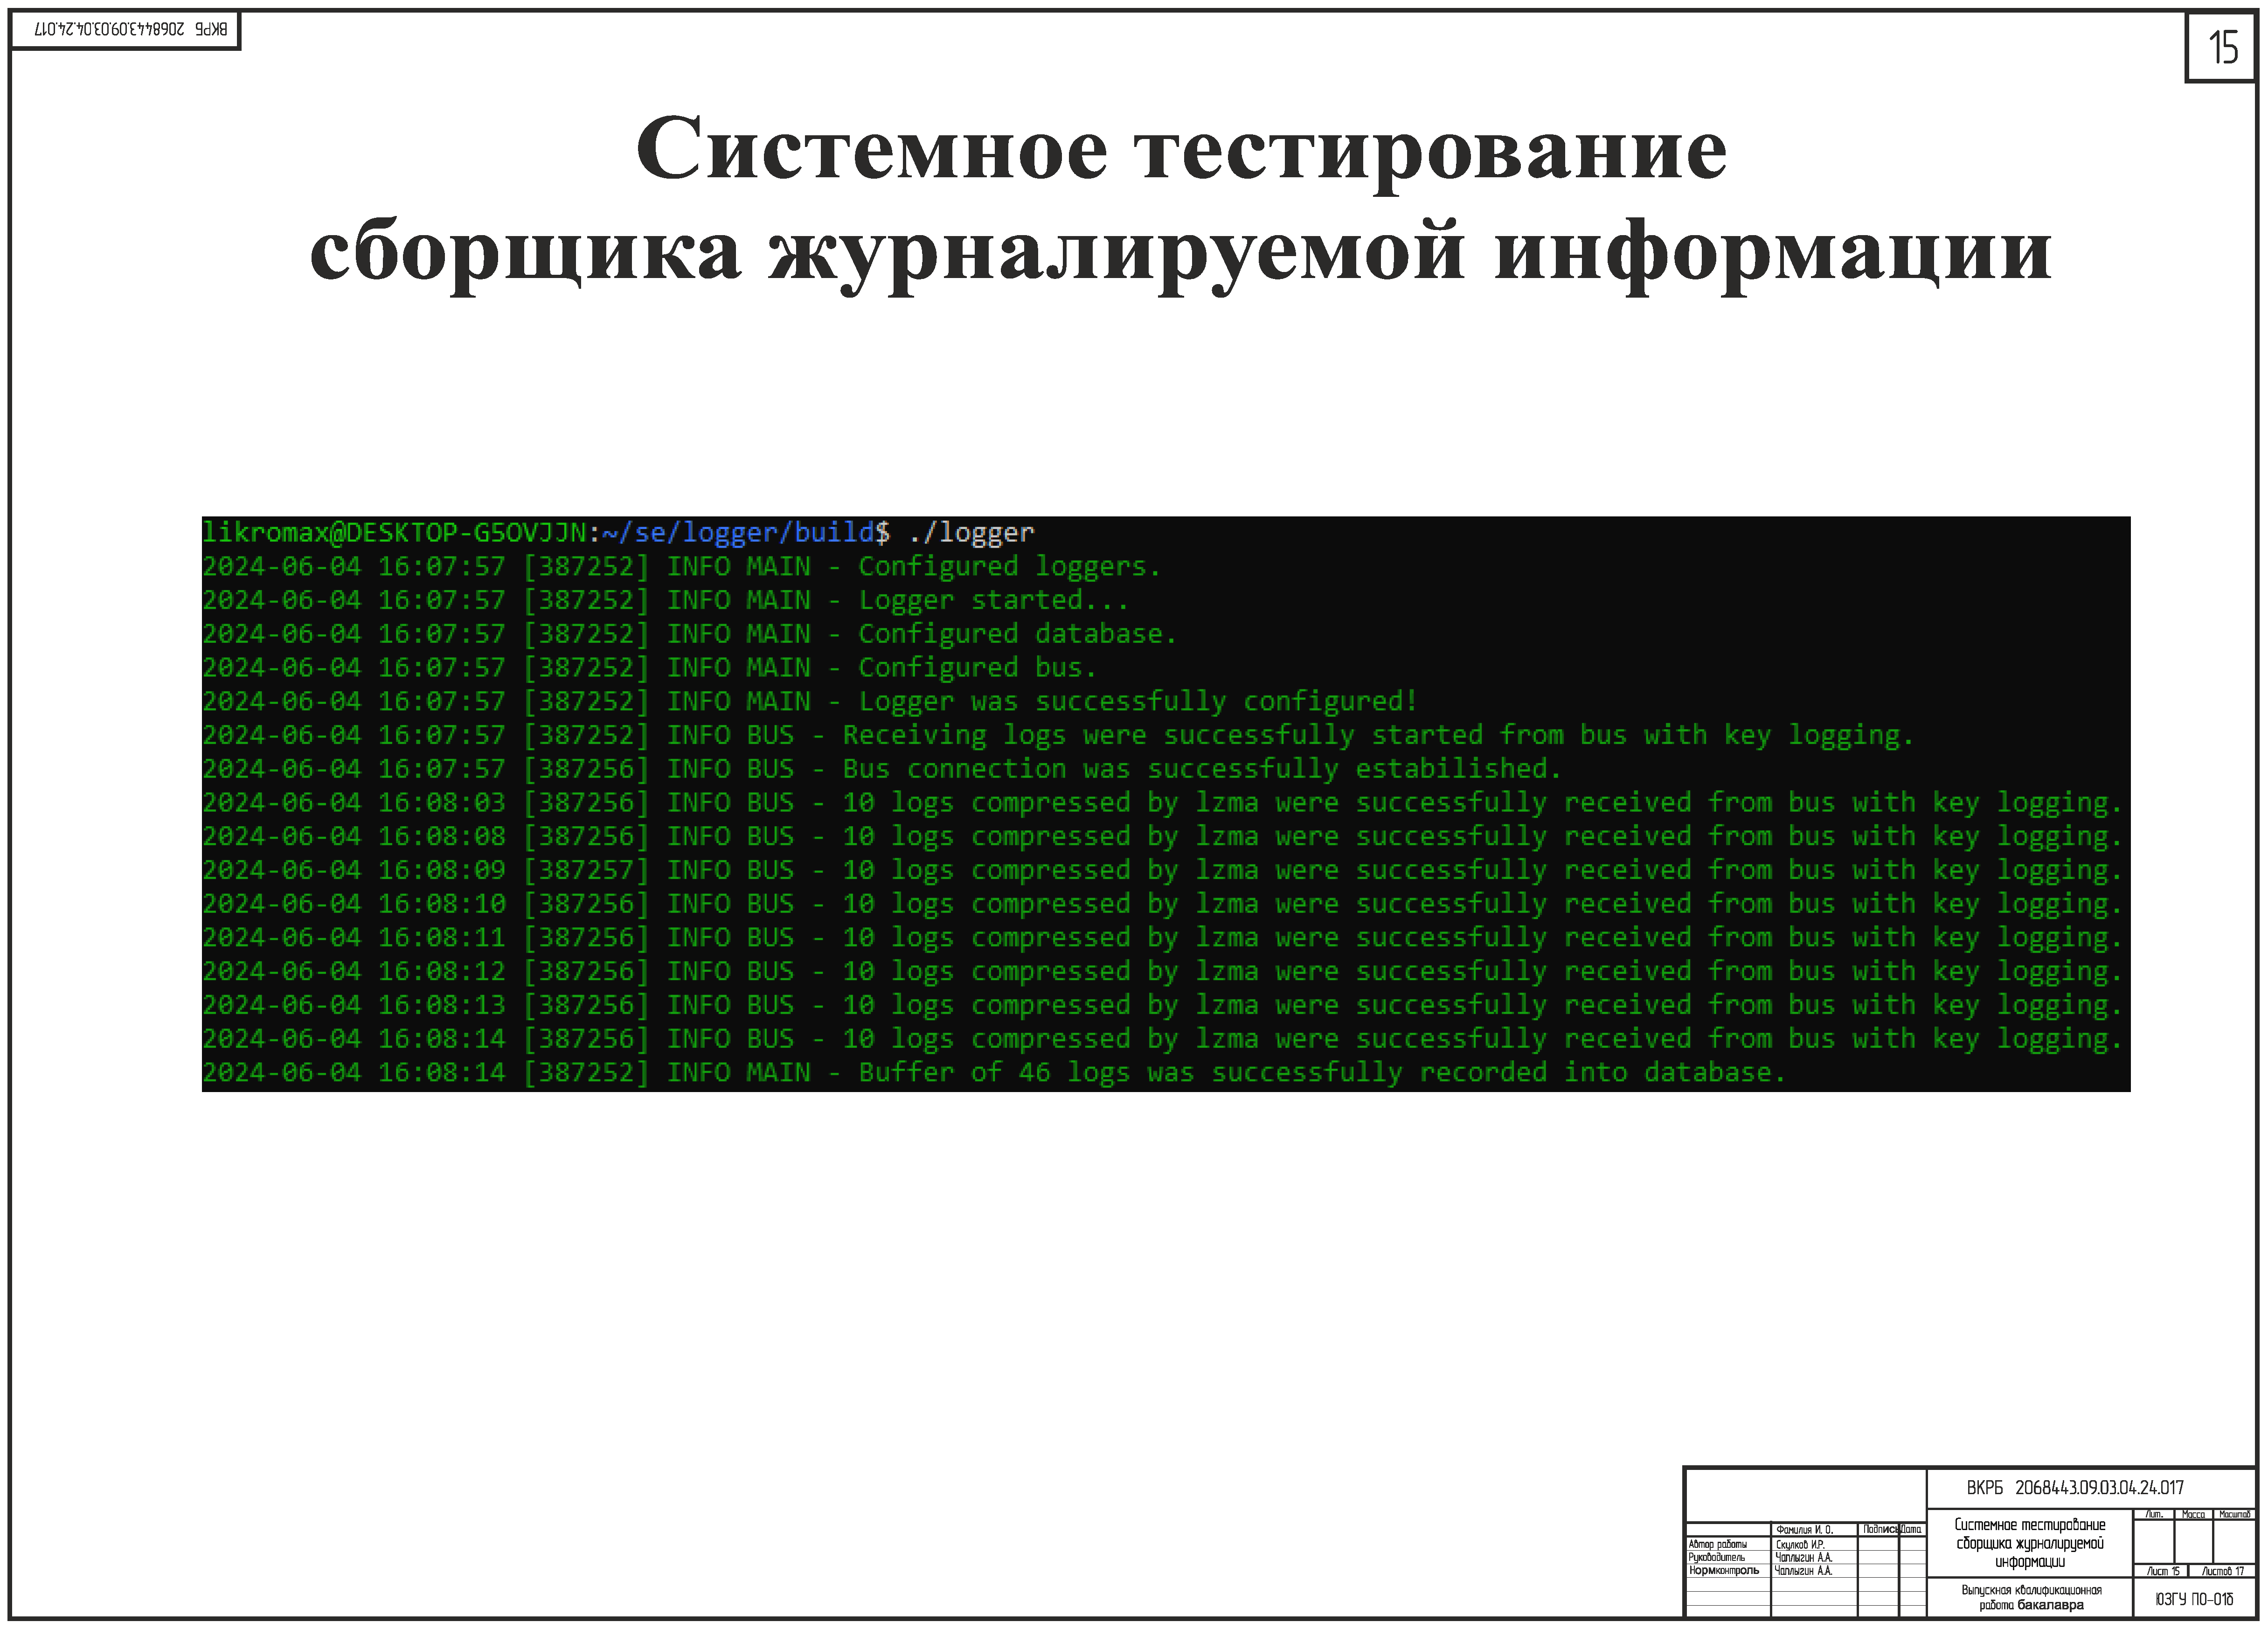
\includegraphics[width=0.82\linewidth]{posters/ptl.eps}
    \заголовок{Системное тестирование сборщика журналируемой информации}
    \label{ptl:image}      
\end{плакат}

\begin{плакат}
    
\includegraphics[width=0.82\linewidth]{posters/ptw.eps}
    \заголовок{Системное тестирование веб-интерфейса}
    \label{ptw:image}      
\end{плакат}

\begin{плакат}
    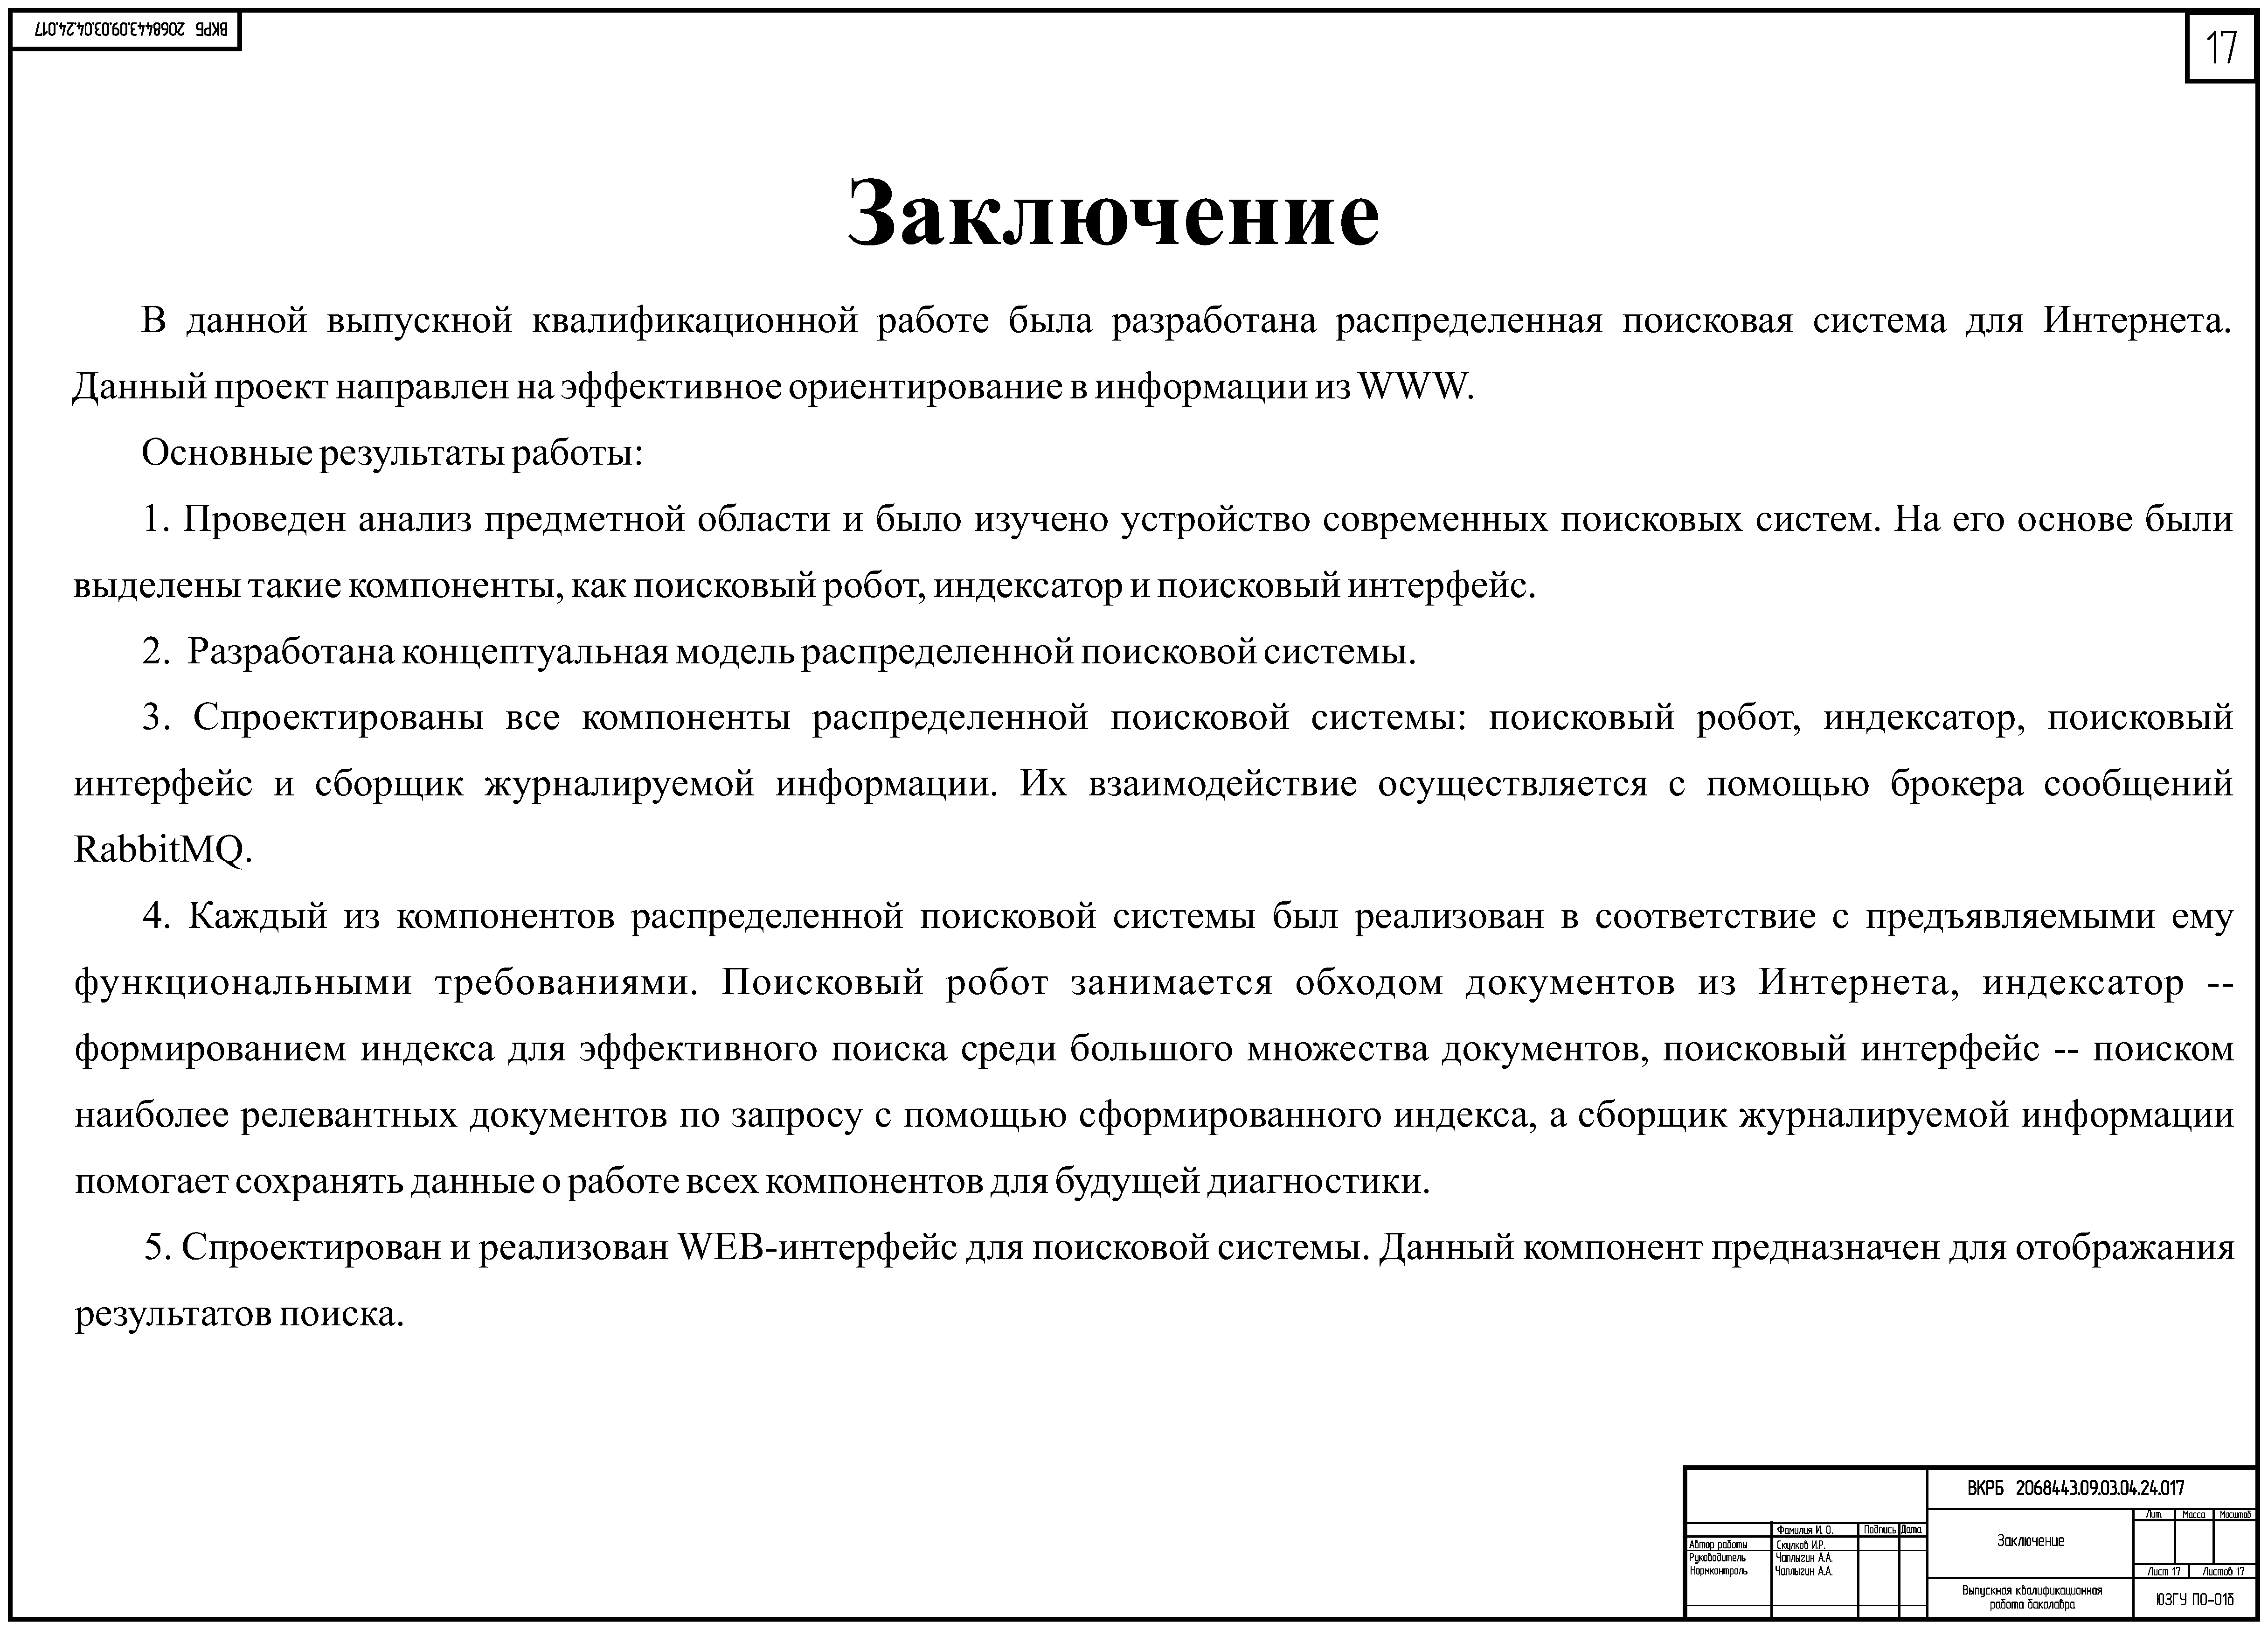
\includegraphics[width=0.82\linewidth]{posters/p6.eps}
    \заголовок{Заключение}
    \label{p6:image}      
\end{плакат}

\end{landscape}